\chapter{Radiogenic backgrounds in LZ}
\label{chap:chap3}

The understanding of backgrounds and their origin in a low-background dark matter detector is critical for the search for dark matter. Without fully understanding and mapping all background sources, the ability to ascribe a statistical significance on any potential excess becomes ever more difficult. Moreover, this understanding is extremely important in sourcing detector materials, strategising cleanliness protocols for construction, and approximating the expected background rates for a potential search. This chapter will discuss background sources in LZ and their origin, highlighting the techniques used for the extensive screening campaign for material selection and detector construction.  

%%------------------------------$$
%%------------------------------$$
\section{Overview}

The backgrounds as seen by the LZ detector can predominantly be characterised under two classes: electron recoils that occur when radioactive species interact with the electrons of the xenon target; and nuclear recoils, which occur when species interact with the nucleus of the xenon target. WIMPs are expected to scatter via nuclear recoils, hence any background that undergoes this type of interaction is WIMP-like, thus has the largest impact to WIMP sensitivity. Although electron recoils can be discriminated to a degree, recombination fluctuations as described in section \ref{subsec:s1} can lead to ER leakage into the NR band. Therefore, any and all sources that contribute towards ER and NR backgrounds are subject to extensive examination before and during detector construction.

The sources of backgrounds contributing to overall ER and NR rates can be categorised as those that are internal and external to the detector. Internal backgrounds are defined to be those that are locked into the detector; originating from fixed material contaminants, surface contaminants and xenon contaminants. External backgrounds include those from laboratory and cosmogenics. This chapter will predominantly focus on fixed contaminants, surface contamination and contributions from the laboratory. Backgrounds from radon emanation---a dispersed xenon contaminant---will later be discussed in detail in chapter \ref{chap:chap4}. Additional backgrounds, such as those from solar and atmospheric neutrino, or the double-beta decay of \XeOTSeven{} are search specific and will become more relevant in chapter \ref{chap:chap5}.

To achieve design sensitivity to a WIMP-nucleon cross section below $ 3 \times 10^{-48} \; \MathText{cm}^{2}$, LZ requires very low radio-contaminants, both intrinsic to materials and as a result of environmental exposure. At an early stage of the project, a requirement of 0.4 NR counts and below 1 \micro{}dru (event/kg/day/keV) of ER background was set for single scatter rates within the fiducial volume and WIMP search energy range from fixed contamination in the detector components. The LZ radioassay program was constructed to screen and source the most radio-pure materials available. The techniques used in the screening process include various forms of gamma and mass spectroscopy; to probe the intrinsically locked radiogenic species. Furthermore, upon completion of material selection, material handling in the transportation and construction process is of great importance in reducing surface contamination. The following sections will give an introduction to the origin of these backgrounds, the techniques used to screen, and the cleanliness protocols developed to monitor and keep surfaces clean in the construction process. 

%%------------------------------$$
%%------------------------------$$
\section{Background Origins}
\label{sec:background_origins}

\subsection{Fixed Contaminants}
\label{subsec:fixed_contaminants}

Naturally occurring radioactive species are often embedded in raw materials with unknown levels of activity. The most prevalent are those of \UTTE{}, \UTTF{}, \ThTTT{} and their progeny, which eventually decay down to a stable isotope of lead via the emission of multiple \alpha{}, \beta{} and subsequent \grays{}. The \UTTE{} and \ThTTT{} chains are particularly dangerous as they often lead to electron and nuclear recoils within the WIMP energy region of interest, the latter through (\alpha, n) reactions within detector materials. 
Measuring the entirety of these chains present a challenge as they contain a number of isotopes with half-lives ranging from milliseconds to billions of years. Often it can be assumed that these chains are in secular equilibrium; a situation that arises due to the relatively long half-lives of parent nuclei in comparison to their daughter nuclei. Hence, a measurement of the activity in one part of the chain can be used to infer the activity of the rest. 
However, \UTTE{} and \ThTTT{} chains, as shown in figure \ref{fig:u_238_and_th_232} are divided into \textit{early} and \textit{late} chains, representing the activity of U/Th as approximated by measurements on isotopic decays above or below the radium isotope on both chains. This distinction is particularly important for \UTTE{} as the \RaTTS{} has a half-life of 1600 years; hence a breakage in secular equilibrium due to a chemical process will take thousands of years to be restored. \UTTEe{} will refer to the \UTTE{} activity as measured above \RaTTS{}, and \UTTEl{} will represent the activity measured from \RaTTS{} and below. A similar approach is taken for \ThTTT{}, with \ThTTTe{} and \ThTTTl{} representing activities above \RaTTE{} isotope and the latter part of the chain.
%
\begin{figure}[t!]
    \begin{center}
        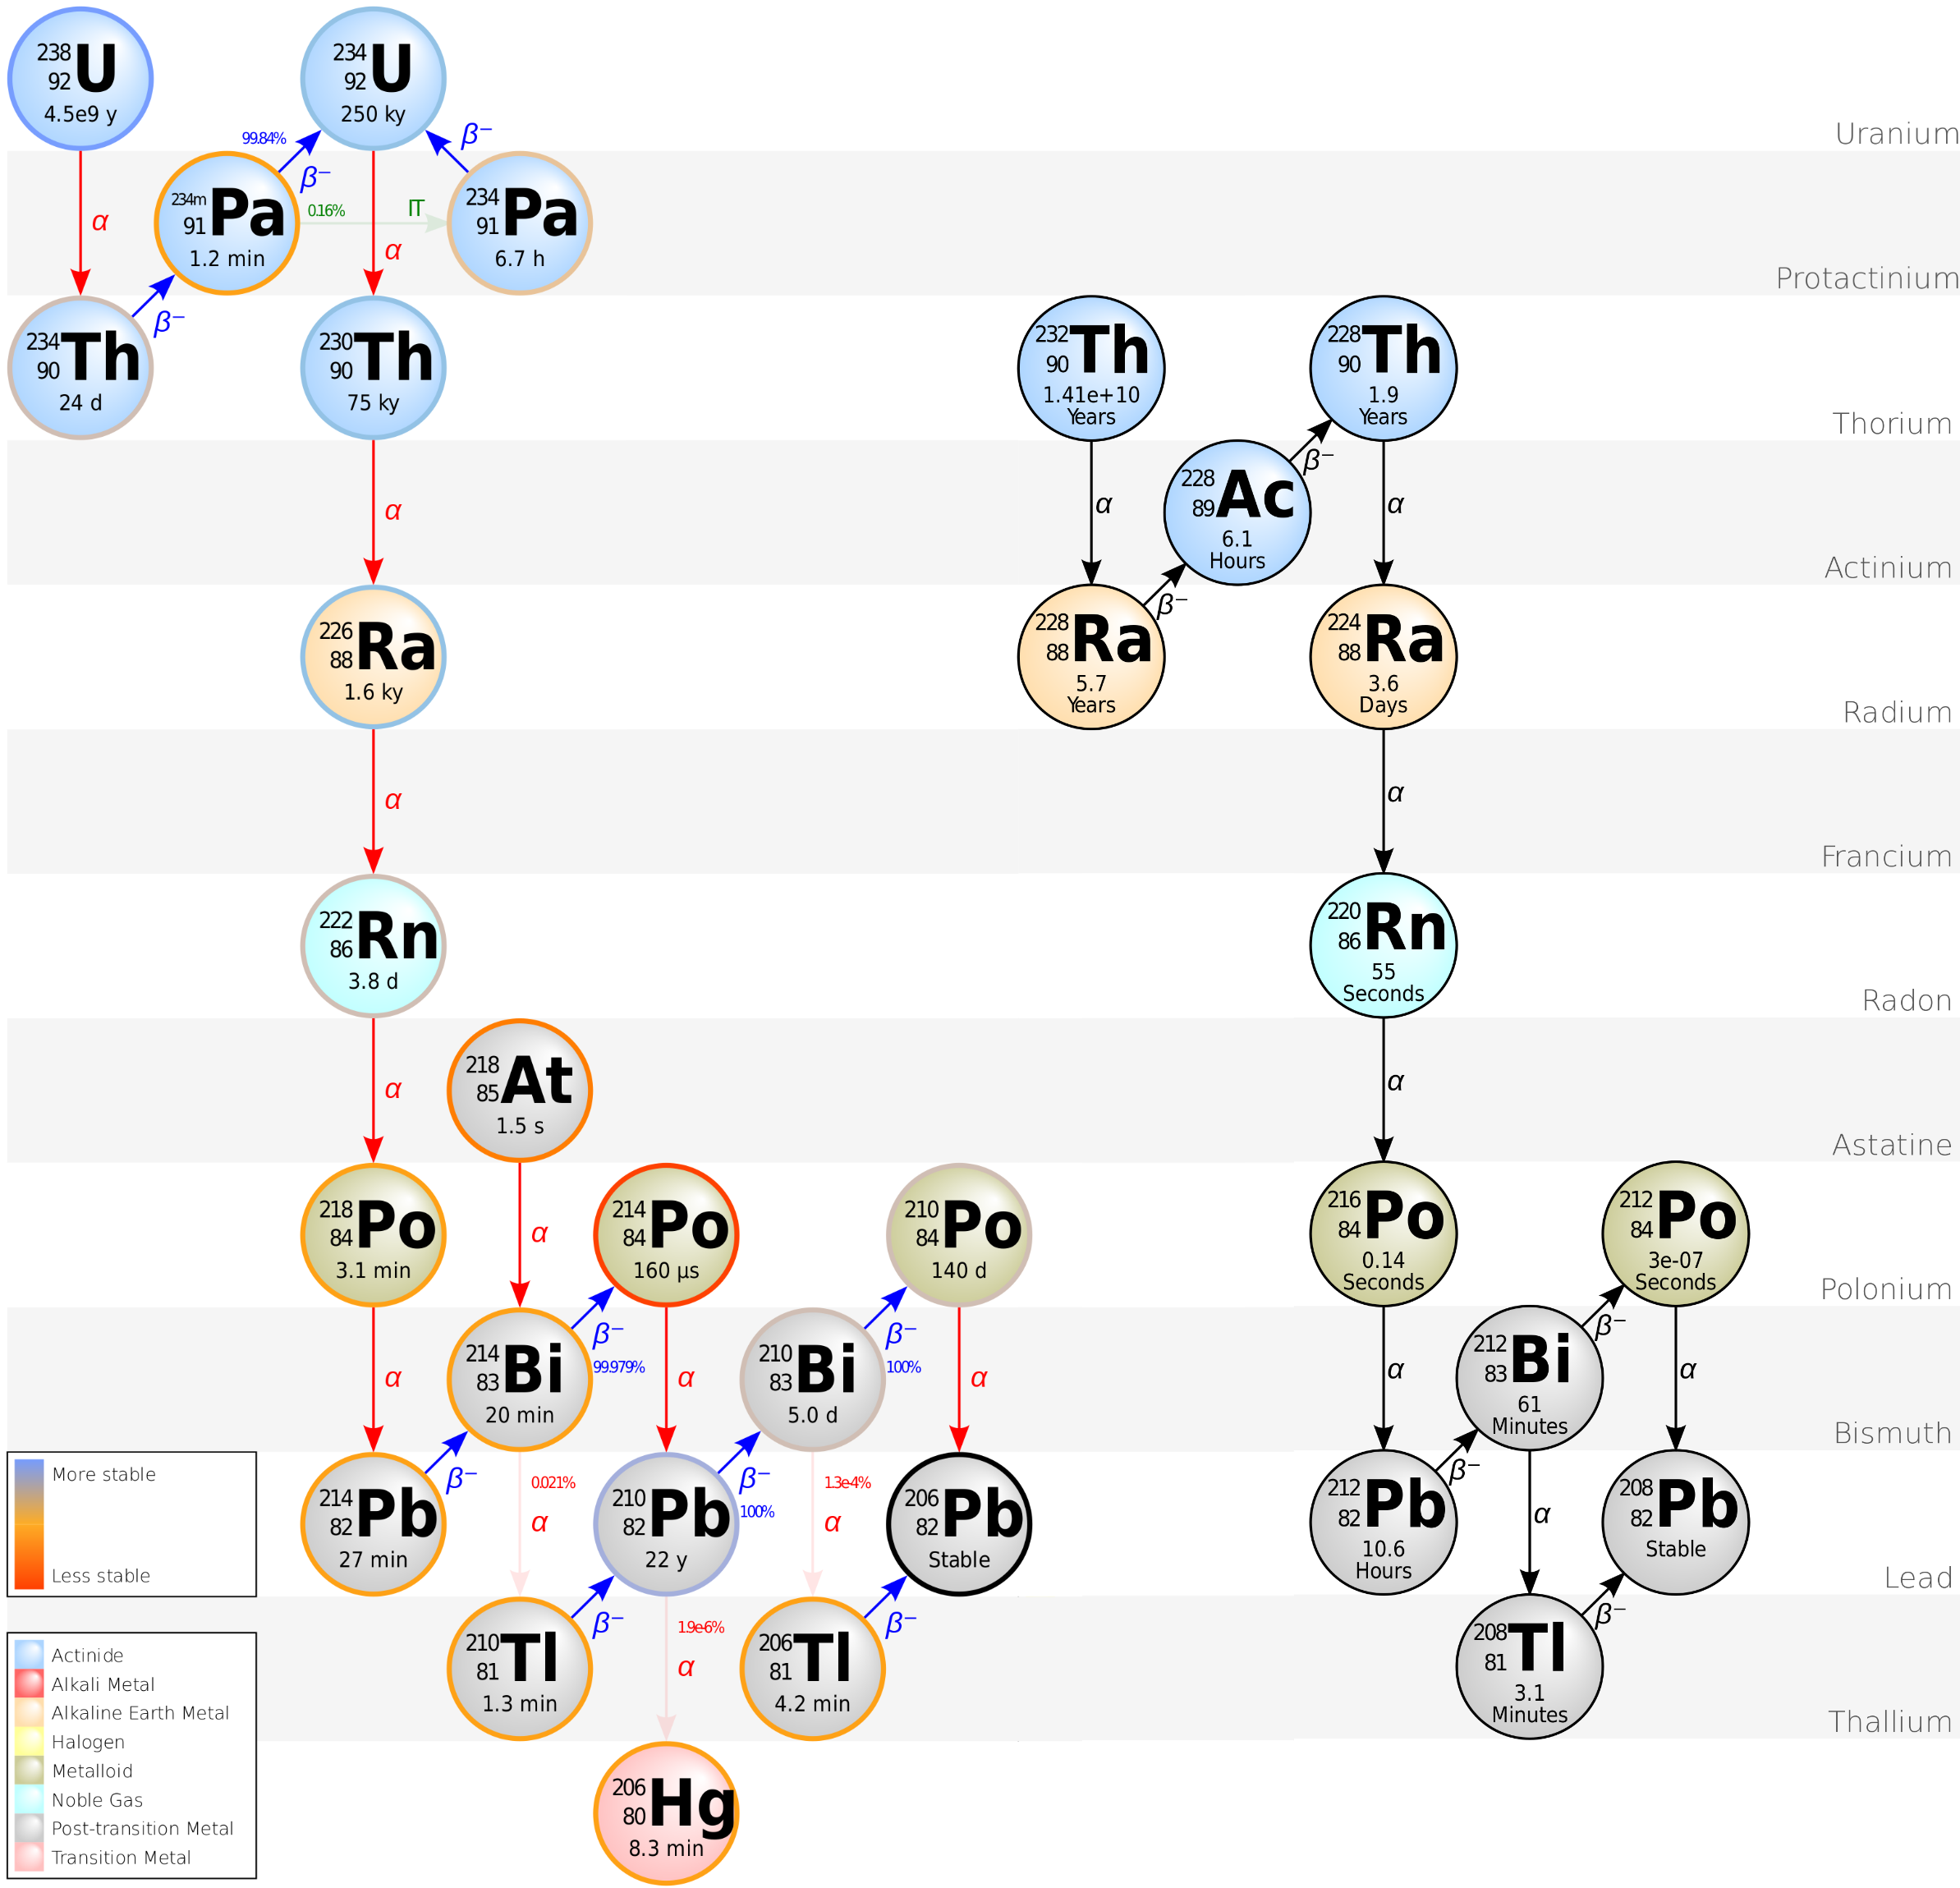
\includegraphics[scale=0.75]{Chapter_3/Figures/U_Th_Chain.png}
        \caption[Isotopes if the \UTTE{} and \ThTTT{} decay chains, detailing their half-lifes and decay types.]%
        {Isotopes of the \UTTE{} and \ThTTT{} decay chains, detailing their half-lifes and decay types. Its important to note that this is a simplified diagram and decays detailed here may occur through other mechanism.}
        \label{fig:u_238_and_th_232}
    \end{center}
\end{figure}
%


Furthermore, \gray{} emitting isotopes such as \KFZ{}, \CoSZ{} and \CsOTS{} are also present in many materials and are a part of the material screening process. \KFZ{} is present within natural potassium at levels of 0.012\%, whereas \CoSZ{} can be produced via neutron activation of naturally occurring \CoFN{}, and \CsOTS{} is often formed as one of the more common fission products by the nuclear fission of \UTTF{}. While these isotopes are often identified and measured by their \gray{} emissions, they all emit \beta particles at range of energies, with the highest endpoint of 1.311 MeV from the \beta-decay of \KFZ{}. Hence, they often result in electron recoils with a wide energy spectrum.

\subsection{Surface Contaminants}
\label{subsec:surface_contaminants}

Fixed contaminants as highlighted in section \ref{subsec:fixed_contaminants} are naturally found in materials, with their isotopic activities expected to stay constant from the point of screening, to their implementation and usage inside the detector. This however does not hold true if a chemical process was conducted between the period of screening and construction. In addition, there are other mechanisms at play which can change the global activity of a material through surface contamination.

Contamination of surfaces can take place whenever a detector material is exposed. Contamination can occur through multiple mechanisms: contamination due to exposure to other material, environmental dust, and isotopic plate-out. However, the specific isotope of importance is the \PbTOZ{} ($\tau_{1/2} = 22.3 \; \MathText{y}$) isotope in the \UTTE{} decay chain. Due to the relatively long half-life of \PbTOZ{}, the isotope can serve as another point of breakage in secular equilibrium. Material exposure to air with \RnTTT{} can result in the plate-out of radon daughters onto surfaces \cite{Bruemmer_2015, Stein_2018}. This process serves as a mechanism to increase the activity of \PbTOZ{} relative to the intrinsic activity driven from fixed contamination. Exposure to other materials, and more importantly environmental dust, can also yield as a mechanism to increase the activity of isotopes in the late chain. The later contaminant not only increases the activity of \PbTOZ{}, but the entire late chain, as the dust particulates will be locked into surfaces with specific concentrations of \UTTE{} and \ThTTT{}.

Plate-out and dust accumulation leads to the generation of both ER and NR backgrounds. ER backgrounds originate from the \PbTOF{} naked betas in the \RnTTT{} sub-chain, leading to a continuous ER background down to the WIMP energy window. NR backgrounds are increased due to the increase in the \alpha-rate, which in turn increases the rate of \alphaN{} processes that release neutrons into the xenon. Furthermore, \PoTOZ{} ions from the \PbTOZ{} sub-chain originating at the edge of the TPC are likely to be misreconstructed as NRs within the fiducial volume. \PoTOZ{} on material surfaces will recoil into the LXe volume producing a complicated wall background (0 to 103 keV in energy). The impact of the latter depends critically on the performance of position reconstruction and drives the 4 cm radial fiducial volume cut. LZ has instituted a target for plate-out of \PbTOZ{} and \PoTOZ{} of less than 0.5 mBq/m$^{2}$ on the TPC walls and below 10 mBq/m$^{2}$ everywhere else. LZ has also instituted a requirement limiting generic dust contamination to less than 500 ng/cm$^{2}$ on all wetted surfaces in the detector and xenon circulation system. 

\subsection{Other Source Origins}
\label{subsec:other_bkkg_sources}

\subsubsection{Xenon Contaminants}

Natural xenon includes trace levels of \KrEF{} and \ArTN{}, both of which disperse throughout the liquid and are \beta{}-emitters that lead to ER events in the ROI. To reduce the levels of \KrEF{} within the LZ xenon, a purification campaign using chromatography to remove krypton from xenon has been implemented \cite{lz_tdr}. The system has been shown to reduce \KrNAT{}/Xe concentration to 0.075 ppt g/g. A further reduction in the levels of argon has also been observed, with an expected concentration of \ArNAT{}/Xe below 0.45 ppb g/g.

Cosmogenic activation of xenon isotopes can also lead to an overall increase in  background rates. The activation rate depends heavily on the depth at which the xenon is stored, as more activation is expected at sea level due to the cosmic ray flux. The equilibrium decay rate of \XeOTSeven{} ($\tau_{1/2} = 36.4 \; \MathText{d}$), a cosmogenic background, was measured by LUX to be ($2.7 \pm 0.5$) mBq/kg after xenon was exposed to cosmic rays on the Earth’s surface \cite{radiogenic_muon_lux}. Further contaminants include \XeOTNm{} ($\tau_{1/2} = 8.9 \; \MathText{d}$), \XeOTOm{} ($\tau_{1/2} = 11.9 \; \MathText{d}$) and \XeOTT{} ($\tau_{1/2} = 5.3 \; \MathText{d}$). Due to their short half-lives, a short cooling period ($\sim$8-months) of the xenon underground before data taking reduces this background significantly. 


\subsubsection{Cosmogenic Activation of Materials}

Cosmogenic activation can also impact detector materials, especially during the sourcing and construction phase, which predominantly takes place in the Earth's surface. At SURF, the location of LZ operations, the muon flux was measured at ($1.149\pm0.017$)$\times10^{-2}$ s$^{-1}$cm$^{-2}$sr$^{-1}$ \cite{surf_muon_flux}. The primary concern from cosmogenic material activation is the production of \ScFS{} ($\tau_{1/2} = 83.8 \; \MathText{d}$). Generated by either muon capture or an \alphaN{} reaction in titanium, \ScFS{} decays via a \beta{}-decay with an endpoint energy 0.357 MeV, with a subsequent emission of two \grays{} of energies 889 keV and 1,121 keV. The production and the decay modes are given as,
%
\begin{equation} \label{eq:cosmogenic_activation}
    ^{46}_{22}\MathText{Ti} + \mu{}^{-} \; &\rightarrow \; ^{46}_{21}\MathText{Sc} + n + \nu{}_{\mu{}}, \\
    ^{46}_{22}\MathText{Ti} + n \; &\rightarrow \; ^{46}_{21}\MathText{Sc} + p, \\
    ^{46}_{21}\MathText{Sc} \; &\rightarrow \; ^{46}_{22}\MathText{Ti} + e^{-} + \nu{}_{e}.
\end{equation} 
%


\subsubsection{Muon-Induced Neutron Background}

Despite 4850-foot (4300 m w.e.) of Earth sitting above the Davis laboratory at SURF, although suppressed in comparison to surface level, a muon flux of ($4.4\pm0.1$)$\times10^{-9}$ s$^{-1}$cm$^{-2}$ is still present \cite{muon_davis}. In detector material and xenon, this flux generally generates internal backgrounds as discussed above. In the laboratory, neutrons from muon-induced electromagnetic and hadronic cascades within the cavern walls can generate background events. The neutron flux from the laboratory walls have been estimated using simulations of muon transport through rock around the laboratory and detector geometry. Attenuation through the water tank and the outer detector scintillators reduces the integrated neutron flux by more than 6 orders of magnitude \cite{TOMASELLO201070} resulting in a negligible contribution to backgrounds in LZ. Its important to note that this mode of background generation may become more significant, if experiments were running closer to the surface.


%%------------------------------$$
%%------------------------------$$
\section{Fixed Contaminant Screening Techniques}
\label{sec:fixed_contaminant_screening}

Approximating and modelling the expected backgrounds originating from fixed contaminants, as covered in detail in section \ref{subsec:fixed_contaminants} has been a high priority for the LZ experiment; initially in selecting radio-pure material for the LZ detector, but also to inform the background model through a combination of screening results, attained from many different screening techniques and detector. The ability to radioassay materials to ever increasing levels of sensitivity, within a short time period is of great importance as the next-generation low-background experiments are probing evermore sensitive parameter spaces. 

In screening for fixed contaminants, the LZ screening campaign has made use of various techniques, including but not limited to an array of high-purity germanium (HPGe) detectors and inductively-coupled plasma mass spectrometry (ICP-MS). The following sections will summarise these techniques within the scope of LZ; focusing on the Boulby underground germanium suite (BUGS) \cite{bugs_boulby} and the ICP-MS facility at University College London (UCL) \cite{icpms_ucl}. 


\subsection{High-Purity Germanium Screening}
\label{subsec:HPGe}

Gamma ray spectroscopy is a technique that uses the principles of interaction of gamma radiation with matter to interpret and measure the activities of specific radio-isotopic impurities within material. The incoming \gray{} photons often deposit their energy by transferring up to all of its energy to the absorbing material through the mechanisms of photoelectric absorption, Compton scattering and pair production. The resultant secondary particles, often electrons, will then induce excitation and ionisation within the material to elude to the nature of the incoming photon. There are various different absorption material, detector design and types of operation to probe a wide range of photon energies but, the primary focus in this section will be germanium semiconductor diodes detectors. Details into the wider theoretical and practical use cases of \gray{} spectroscopy are provided in \cite{gilmore2011practical}.

\subsubsection{Germanium Detectors}

Germanium detectors are a class of semiconductor detectors that are widely used in \gray{} spectroscopy. Their relatively high atomic number, Z; capacity for large crystalline growth with impurity levels of $10^{10} \; \MathText{atoms/cm}^3$ or lower; and the energy resolution achieved due to their very low bandgap ($E_{g} \approx 1 \; \MathText{eV}$), make them a prime candidate for keV--MeV \gray{} detection. 

The periodic lattice formation in germanium crystals lead to distinct band formation for electrons that exist within the solid. The \textit{valence band} corresponds to outer-shell electrons that form covalent bonds within the crystal; the \textit{conduction band}, sitting at a higher energy level, represents the band in which electrons are free to migrate through the crystal. The excitation of an electron from the valence band to the conduction band often takes place due to thermal energy. In doing so, it places an electron into the conduction band that is free to drift, but also creates what's known as a vacancy (hole) in the otherwise full valence band---the combination of these is called an \textit{electron-hole} pair. The electron in the conduction band and the subsequent hole can both be drifted if an electric field is applied to the crystal; though in opposite directions, as the hole represents a net positive charge. The resultant drifted charge is then collected using electrodes.

The electrical properties of commercial crystals is often dominated by the small residual impurities that remain within such crystals. The nature of these impurities determine the type of semiconductor present; often labeled as an \textit{n}- or \textit{p}-type. In \textit{n}-type crystals, the impurities occupy sites within the lattice and have extra valence electron in their outer-shell. Often referred to as \textit{donor impurities}, they readily contribute electrons to the conduction band. In such material, the majority charge carriers are electrons. In \textit{p}-type, the impurities often have one less valence electron relative to the crystal, effectively increasing the number of holes within the entire crystal. Referred to as \textit{acceptor impurities}, these sites capture electrons excited to the conduction band; hence the majority charge carrier in such material are the excess holes that are formed within the material. Materials can often be doped with specific impurities to determine the nature of the crystal.


\subsubsection{Boulby Underground Germanium Suite (BUGS)}

The Boulby Underground Germanium Suite (BUGS) hosts seven gamma spectroscopy detectors, 1.1 km underground, at the Boulby Underground Laboratory in a class 1000 cleanroom, constructed and developed primarily for LZ. Since 2013, majority of the gamma spectroscopy screening efforts in LZ were conducted by the Chaloner (Mirion BE5030 broad-energy ultra-low background (ULB) HPGe detector), Lunehead (Mirion ULB SAGe well-detector), and Lumpsey (Ortec p-type detector) detectors. In addition to these detectors, BUGS has installed additional Mirion \textit{specialty ultra-low background} (S-ULB) detectors which have been used to screen later LZ samples since 2017. These comprise two p-type detectors, Belmont and Merrybent, with relative efficiencies of \SI{160}{\percent} and \SI{110}{\percent}, respectively, and Roseberry, a BE6530 BEGe type detector.

The shielding of such detectors is detrimental to their operational output. The idea behind these detectors is to limit the \grays{} hitting the crystals strictly to those originating from the sample of interest. \grays{} originating either from detector material or external sources are considered to be background. The BUGS detectors are housed in custom shields designed and built by Lead Shield Engineering Ltd. The shields comprise 9 cm thickness of lead and 9 cm thickness of copper with interlocking retractable roofs to simplify sample loading. The lead used in these shields has mostly been recycled from lead used to shield previous low-background experiments hosted at the Boulby Underground Laboratory. The characterizations and sensitivities of these detectors are discussed in \cite{bugs_boulby}.

\grays{} originating from the \RnTTT{} sub-chain in the air can also contribute towards the background rate. To reduce such background, the shields used for all detectors are purged using nitrogen from a Wirac NG6 gas generator. The Boulby Underground Laboratory benefits from a low baseline radon level (averaging $\sim2.5 \; \MathText{Bq/m}^3$). To remove residual radon in the nitrogen purge gas, charcoal traps containing approximately 6 kg of Carboact activated charcoal are deployed in a Labcold ULTF416 -80$^{\circ}$C chest freezer. This radon reduction system is based on the design of a radon emanation detector developed at the Centre de Physique des Particules de Marseille (CPPM)~\cite{Noel:2015nla}. 


\subsubsection{Other \gray{} Screening Facilities for LZ}

Other than BUGS, LZ employs various other \gray{} screening facilities, including the Black Hills Underground Campus (BHUC) \cite{Mount:2017iam}, located at the 4850-foot level of SURF, which hosts a class 2000 clean-room containing seven low and ultra-low background HPGe detectors; the Lawrence Berkeley National Laboratory (LBNL) \cite{Smith:2015aoa}, which operates two HPGe detectors devoted to assay; and University of Alabama operating two above-ground Canberra p-type low-background HPGe detectors \cite{Tsang:2019apx}.

The LZ radioassay program uses a total of 12 detectors from the facilities mentioned above. A more detailed description of these facilities and their housed detectors can be found in \textit{The LUX-ZEPLIN (LZ) radioactivity and cleanliness control programs} paper \cite{lz_screening}. A summary of the 12 detector used by LZ, detailing the type of detector and some key characteristics can be found in table \ref{tab:GeDetInf}.

\begin{table}[h]
\centering
\caption
[Key characteristics of the 12 detectors used in the LZ HPGe screening campaign.]
{Key characteristics of the 12 detectors used in the LZ HPGe screening campaign. Crystal mass and volume is included to give an idea of the relative sizes of the crystal. In addition the relative efficiency is given for the p-type detectors and the area of the front face is given for the BEGe detectors \cite{lz_screening}. For historical reasons, the relative detection efficiency of coaxial
germanium detectors is defined at 1.33 MeV relative to that of a standard 3" diameter by 3" long NaI(Tl) scintillators.}
    \label{tab:GeDetInf}
    \vspace{1mm}

    \renewcommand{\arraystretch}{1.2}
    \begin{tabularx}{1.0\linewidth}{@{\extracolsep{\fill}}lllcccc}
    \toprule
    
    \multirow{3}{*}{\textbf{Location}} & %0
    \multirow{3}{*}{\textbf{Detector}} & %0
    \multirow{3}{*}{\textbf{Type}} & %1
    \multirow{2}{*}{\textbf{Volume}} & %2
    \multirow{2}{*}{\textbf{Mass}} & %3
    \textbf{Relative} & %4
    \textbf{Face} %5
    \\
    &
    & %0
    & %1
    \multirow{2}{*}{\textbf{[cm$^{3}$]}} & %2
    \multirow{2}{*}{\textbf{[kg]}} & %3
    \textbf{Efficiency} & %4
    \textbf{Area} %5
    \\
    &
    & %0
    & %1
    & %2
    & %3
    \textbf{(\%)} & %4
    \textbf{[cm$^{2}$]} %5
    \\
    \hline
    \hline

    \multirow{6}{*}{BUGS} & Belmont & p-type & 600 & 3.2 & 1.92 & - \\
    & Merrybent & p-type & 375 & 2.0 & 1.87 & - \\
    & Lunehead & p-type & 375 & 2.0 & 1.86 & - \\
    & Roseberry & BEGe & 170 & 0.9 & - & 181.1 \\
    & Chaloner & BEGe & 150 & 0.8 & - & 1053.0 \\
    & Lumpsey & SAGe well & 263 & 1.4 & - & - \\
    \hline
    LBNL & \textsc{Merlin} & n-type & 430 & 2.2 &3.59 & - \\
    \hline
    \multirow{4}{*}{BHUC}& \textsc{Maeve} & p-type & 375 & 2.0 &3.19 & - \\
    & \textsc{Morgan} & p-type & 375 & 2.0 & 2.68 & - \\
    & \textsc{Mordred} & n-type & 253 & 1.3 &2.44 & - \\
    & SOLO & p-type & 113 & 0.6 & 5.52 & - \\
    \hline
    \multirow{2}{*}{Alabama} & Ge-II  & p-type & 260 & 1.4 & 3.6  & - \\
    & Ge-III & p-type & 406 & 2.2 & 2.71 & - \\
    
    \bottomrule
    \end{tabularx}
\end{table}


\subsubsection{HPGe Cross-Calibration}

\begin{table}[t!]
\centering
\vspace{-5mm}
\caption{Results from the HPGe cross-calibration performed using a sample of Rhyolite. For the \utTeE{} and \utTeL{} columns, the contamination reported is that of the progenitor isotope \utTe{} assuming secular equilibrium and for the \thtTtE{} and \thtTtL{} columns, the contamination reported is that of \thtTt{} assuming secular equilibrium.}
    \label{tab:GeCrossCal}
    \renewcommand{\arraystretch}{1.1}
    \begin{tabular}{lccccc}
    
    \textbf{Detector} & %0
    \textbf{\utTeE{} (ppm)}  & %1
    \textbf{\utTeL{} (ppm)} &  %2
    \textbf{\thtTtE{} (ppm)} &  %3
    \textbf{\thtTtL{} (ppm)}  & %4
    \textbf{K ($\%$)}   \\  %5
    
    \hline
    \hline
    
    Reference & 8.87(4) & 8.5(1) & 12.1(1) & 12.1(1) & 2.82(1) \\
    
    \hline
   
    \textsc{Merlin} & 8.92(9) & - & 12.4(1) & 12.4(1) & 2.81(3) \\
    \textsc{Maeve} & 8.6(1) & 8.6(1) & 11.9(1) & 11.9(1) & 2.74(3) \\
    \textsc{Mordred} & 7.92(5) & 10.2(1) & 11.3(2) & 11.3(1) & 2.66(6) \\
    SOLO & 6.16(1) & - & 12.5(7) & 9.94(1) & 2.91(1) \\
    Chaloner & 8.73(5) & 7.9(2) & 11.1(1) & 11.1(1) & 2.81(1) \\
    Lunehead & 8.5(1) & - & 11.8(1) & 11.8(1) & 2.85(1) \\
    Ge-II & 9.6(13) & 11.4(15) & 12(16) & 12.2(17) & 3.4(4) \\
    Ge-III & 9.2(9) & 10.3(10) & 12.1(12) & 12.8(13) & 3.3(3) \\
   
    \hline
   
    Average & 7.61(3) & 9.2(2) & 11.9(1) & 10.54(0.5) & 2.84(2) \\
    Std. Dev. & 0.98 & 1.26 & 0.46 & 0.84 & 0.25 \\
    
    \bottomrule
\end{tabular}
\end{table}

The screened samples in LZ were distributed amongst the 12 detectors detailed in table \ref{tab:GeDetInf}, all with different backgrounds, shielding arrangements and operational history. To evaluate the systematic uncertainties and be able to correlate results from one detector to that of another, a sample of Rhyolite with well-characterized uranium, thorium and potassium content was used for cross-calibration. The material has been used by LBNL for over 30 years, with a well established uniformity across the sample.

An S5 Marinelli beaker of this mineral was prepared and sealed, with the content and its activity unknown to the collaboration. The comparison of results from different detectors uncovered some issues with several analyses, mostly due to problems with the Monte Carlo simulations of the detectors. These issues were identified and corrected without knowledge of the true calibration source material. The results were again compared across all the detectors. It is important to note at this point that when a concentration is reported, in parts per value ($e.g.$ ppm, ppb, ppt) it is no longer pertinent to refer to late chain or early chain values as the concentration defines the concentration of the progenitor isotope (\UTTE{ }, \UTTF{}{}, \ThTTT{}) assuming secular equilibrium~\cite{malling:2013jya}. Table \ref{tab:GeCrossCal} lists reference values for each isotope; compares results from each detector; and gives their combined average and standard deviation. The cross-calibration effort confirmed that the modeling of detector geometries and efficiencies were correctly handled and provides a reasonable estimate on the systematic variation among the assays of \SI{\sim 10}{\percent} thus giving the collaboration confidence that each individual facility is able to produce consistent and accurate assay results.


\subsection{Inductively-Coupled Plasma Mass Spectrometry}
\label{subsec:ICPMS}

Inductively-Coupled Plasma Mass Spectrometry (ICP-MS) allows very precise direct measurement of the elemental abundances of uranium and thorium in small samples. The assays can be very quick, taking hours to days depending on requisite sensitivity down to sub-ppt (\si{\gram} of U/Th per \si{\gram} of material) levels and depending on related sample preparation protocols. ICP-MS has been used extensively in LZ to quickly measure \utTe{} and \thtTt{} in small samples to either reject or clear materials for use, or to pre-screen materials prior to  assay with gamma spectroscopy which can determine the complete activity through the \utTe{} and \thtTt{} decay chains. In addition to constraining systematic uncertainty and directly determining activity at the top of the \utTe{} and \thtTt{} chains, ICP-MS has been used in LZ as part of our QC and QA program to ensure radioactivity and cleanliness compliance through component manufacture and delivery. The speed of ICP-MS allowed for rapid analysis of test pieces provided by manufacturers at specified points in the production processes, to detect potential issues and to ensure radioactivity and cleanliness compliance. 

The majority of ICP-MS assays for LZ were performed using a dedicated mass spectrometry laboratory at UCL, housed in a class 1000 cleanroom facility and operating an Agilent 7900 spectrometer installed in 2015 exclusively for LZ~\cite{icpms_ucl}. Sample preparation and analysis procedures have been developed for materials with U/Th concentrations in the ppt to 1 ppb range. Samples are microwave-digested in pre-cleaned modified-PTFE (TFM) vessels using ultra-high purity acids. They are then diluted, without further chemical treatment, into disposable 50 \milli{}\litre{} polypropylene (PP) vessels ready for ICP-MS analysis. Fractional recoveries of \thtTz{} and \utTT{} spikes added prior to digestion are used to correct for \thtTt{} and \utTe{} signal loss from a range of sources. In particular, this enables accurate analysis of samples with high total dissolved solids (TDS) where the instrument response degrades throughout the run. A full assay including digestion, ICP-MS measurement and analysis can be completed in a single day. The UCL facility was upgraded in 2019 with an Agilent 8900 ICP-MS. 

In addition to the system at UCL, some material samples were assayed using facilities at the University of Alabama, the  Centre for Underground Physics in Korea, and the Black Hills State University.  At the University of Alabama, the LZ group set up a sample preparation laboratory in a Class 500 cleanroom equipped with a cryogenic mill, microwave digestion system, and digestion bomb.  Further processing of samples, including spiking and resin-based extraction of U/Th isotopes was carried out in a separate cleanroom.  The samples were then given to the Department of Geological Sciences which processed the samples using a Perkin-Elmer SCIEX-ELAN 6000 system.  At Korea and Black Hills State, samples were measured using Agilent 7900 spectrometer, as was used at UCL.


%%------------------------------$$
%%------------------------------$$
\section{LZ Cleanliness Protocols \& Surface Contamination}
\label{sec:cleanliness}

Surface contamination through dust and radon daughter plate-out can lead to ER and NR generation as detailed in section \ref{subsec:surface_contaminants}. This class of contamination can take place from the moment a material is manufactured, up until it is mounted onto the detector and protected from exposure. This section will entail dust deposition and plate-out on LZ material, focusing on the protocols used in mitigating against such contamination; techniques used in handling, modelling and estimating exposure rates on critical surfaces of the detector.


\subsection{LZ Cleanliness Protocols}
\label{secsec:cleanliness}

Often, manufacturing of detector components are sourced out to  experienced companies tailored for specialty instrumentation, such as Hamamatsu for PMTs, Loterios for the LZ cryostats and Axon for cables. And in other cases, specific instrumentation was designed and built by some of the universities involved in the project. Despite efforts in monitoring these environments for dust and radon plate-out, levels of contaminants in such environments are well above the baseline contamination requirements of the LZ project. To tackle this issue, most of the detector components after manufacturing were sent to a certified precision cleaning company, AstroPak Inc. The cleaning process involves chemical passivation or electropolishing---both of which are intended to etch surface layers of the material, removing any dust or plate-out isotopes on the surface. After these procedures, the material are sealed with radon-proof bags, either aluminised Myler or Nylon bags with reduction factors of ${2500 \pm 1042}$ and ${130 \pm 3}$, respectively \cite{Meng:2019ker}, and purged under nitrogen gas. The components are then stored safely up until their use-case in the construction process. 

Majority of LZ assembly and construction took place in the surface assembly laboratory (SAL), in SURF. The laboratory was engineered as an ISO 6 class cleanroom with an average particulate count of $\leq 10$ per cubic foot. The air filtration system was fitted with large activated charcoal columns to scrub the radon within the cleanroom to reduce the averaging activity of ambient radon level  $\leq 0.5 \; \MathText{Bq/m}^{3}$. The radon reduced cleanroom (RCR) in particular was designed with a high recirculation rate of 240.7 m$^3$/min in order to sweep out most of the radon daughters---in particularly \PoTOE---before plate-out can occur. The cleanroom was under constant dust and radon monitoring. 

Upon their use-case, the material components were taken into the RCR with their outermost seals removed, inspected for dust by ultra-violate (UV) light and fully un-sealed under de-ionising fans that served to reduce any static buildup, which was shown to be effective in reducing dust accumulation on surfaces. Majority of the critical assembly was then completed under these de-ionising fans. For situations which required further cleaning, non-shedding mini-filament (Abgenics Essence Gold) wipes saturated with \SI{99}{\percent} pure IPA was used as cleaning agents. 

Cleanroom garbs worn by personnel working on the assembly were changed after every work shift and wiped off with a lint roller multiple times during work to remove particulates that could deposit onto detector surfaces. Small detector components were sealed in double nylon bags which prevented plate-out since the components were then no longer in contact with the radon-laden air. Larger components like the cryostat vessels or PMT arrays had bespoke airtight enclosures, enabling additional filtered air and N$_{2}$ purges while in storage within the cleanroom to further mitigate against radon plate-out.


\subsection{Surface Dust}
\label{secsec:surface_dust}

The predominant source of dust that components are exposed to are as a result of outdoor air flowing into the SAL and that carried in from personnel, equipment and material. Dust monitors (Met One GT-526S particle counters) fitted in different locations of the cleanroom indicate increased levels of detection proportional to the activity within the cleanroom. While regular cleaning of the cleanroom and the air filtration system removes most of the dust, some still deposits on surfaces, including some of the most critical regions of the detector, i.e. PMTs and TPC walls. To approximate deposition levels on surfaces and locked in dust amounts, two techniques have been utilised in measuring and modelling surface dust; the use of witness plates and tape-lifts. 


\subsubsection{Witness Coupons}

Witness coupons made of PTFE and glass; cleaned with isopropyl alcohol (IPA) soaked non-shedding wipes are placed in multiple locations within the RCR, serving as controlled surfaces for dust collection. Fresh coupons are often used for specific phases of the construction with the assumption that the coupons would accumulate dust at a similar rate to that of the detector surfaces exposed during that phase of construction. The PTFE and glass coupons are then screened under fluorescence and optical microscopy, respectively, and processed via an ImageJ software \cite{DBLP:journals/corr/RuedenSHDWE17} to reveal smaller particulates to determine the size distributions and their relative contributions to the dust density accumulated on the coupons' surfaces. Once the dust particulates size distribution is determined, as shown in figure \ref{fig:dust_particle}, the dust density accumulated on the coupon (in \si{\nano\g\per\cm\squared}) is calculated by dividing the accumulated mass (assuming particulates are spherical in shape with density of 1${g/cc}$) by the surface area of the coupons. Blank rates from unexposed coupons prepared in the same manner are taken into account in the analyses by background subtraction. The results from witness plates are a good measure on average dust levels during operation but are not precise enough to estimate the actual dust accumulation on surfaces.
%
\begin{figure}[hbt!]
    \centering
    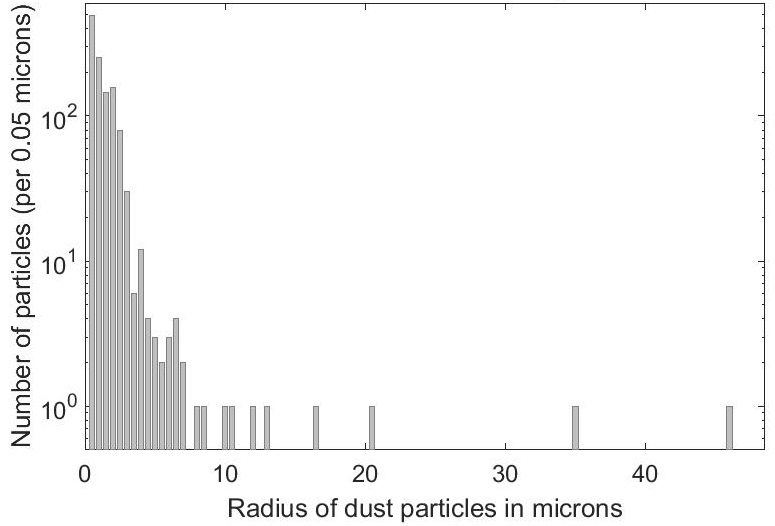
\includegraphics[scale=0.46]{Chapter_3/Figures/ParticlesByRadiusLogScale.jpg}
    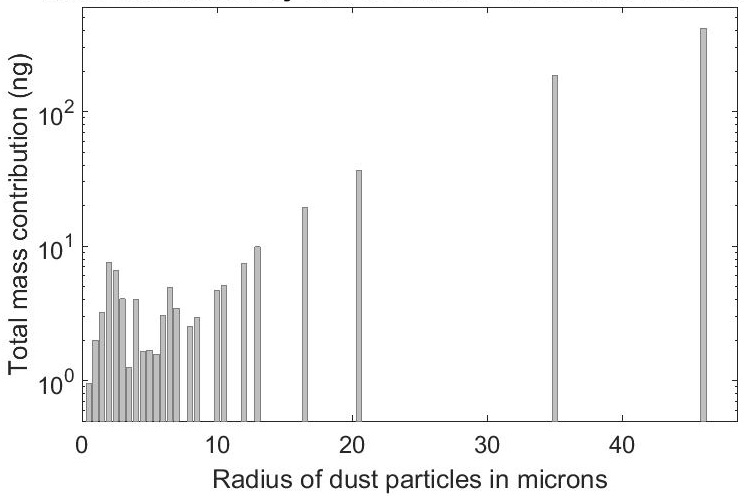
\includegraphics[scale=0.49]{Chapter_3/Figures/MassContributionLogScale.jpg}
    \caption[Dust particulate size and mass distribution from fluorescent image analysis of sample witness plates.]
    {Dust particulate size distribution (left) and mass distribution (right) from fluorescent image analysis of a witness plate. Majority of the mass on the coupon is from a small number of larger particles. Particulates of size $>50 \; \micro{}m$ are rarely recorded.}
    \label{fig:dust_particle}
\end{figure}
%


\subsubsection{Tape-lifts}

In order to fully assess the dust levels on surfaces post-construction, surfaces of detector material were sampled with acetate or carbon tapes. The tapes were applied onto surfaces to remove the accumulated dust and assayed using the same fluorescence microscopy technique utilized for the witness coupons. The choice of tape material depends on the surface roughness of the component; acetate tape works better on smooth surfaces, like PTFE, while, for rougher surfaces like titanium, carbon tapes were found to perform better. However, tape-lifts cannot be taken on particularly sensitive parts of the detector, and therefore, they do not negate the need for coupons, but rather complement them. Both tape-lifts and coupons are necessary for a full history of the dust deposition on every component during the assembly process. 


\subsection{Radon Plate-out}
\label{secsec:radon_plateout}

The presence of primordial \UTTE{} and the effect of radon emanation from the environment can vary radon levels in the air from 5--15 Bq/m$^3$ and to much higher levels in indoor environments. Once in air, the consequent \alpha-decay of \RnTTT{} and daughters can lodge into material surfaces due to the kinetic energy carried as a result of the decay. As described in section \ref{sec:cleanliness}, LZ limits the plate-out rate by assembling most of the background-prone instrumentation from plate-out in the RCR, with a continuous filtration system constantly circulating to reduce the concentrations of \RnTTT{} and daughters in the air. Absolute plate-out prevention is however not possible, and the remaining \PoTOE{} that plates out is problematic due to the long-lived \PbTOZ{} daughter which will decay over time in the detector. Therefore, the estimation of plate-out rates during assembly is crucial for operational control and background modelling.

Plate-out rates onto material are estimated using the Jacobi model \cite{jacobi1972activity, knutson1988modeling}, describing particle deposition on surfaces from a balance of in- and out-flux of concentration in a maximally mixed air model. The model assumes that all surfaces within a given enclosure have equivalent plate-out rates per area, which is a function of air circulation rate, Rn concentration, volume, and surface area within the enclosed space the material surfaces reside. The plate-out rate is given as Becquerel per unit area and time of \PbTOZ{}, where
%
\begin{equation}
    R_p=C_{Rn}\lambda_{Pb_{210}}\frac{\Lambda_d}{(\Lambda_d +\Lambda_v)}\frac{V}{A}.
    \label{eq:jacobi_eq}
\end{equation}
%
The \RnTTT{} concentration as obtained by radon monitors within the RCR (Durridge RAD7) is given by ${C_{Rn}}$, where ${\lambda_{Pb_{210}}}$ is the decay rate of \PbTOZ{}. ${{\Lambda_d =v\frac{A}{V}}}$ is the deposition rate that depends on the diffusion velocity, $v$, of radon daughters measured to be between 5--15 m/h \cite{knutson1988modeling}, ${{\Lambda_v = \frac{R}{V}}}$ is the air ventilation rate obtained by dividing the recirculation rate, $R$, by the volume, $V$, of the cleanroom, and $A$ is the surface area of the RCR at SAL where most of the assembly work has been performed. The ratio, ${\frac{\Lambda_d}{(\Lambda_d +\Lambda_v)}}$, corresponds to the probability that a radon daughter will plate-out before removal through ventilation and is calculated to be 0.17.

In estimating a plate-out rate, the Jacobi model does not differentiate between types of material. This assumption is shown to be incorrect for material with highly negative triboelectric charging---a type of contact electrification on which certain materials become electrically charged---such as PTFE \cite{zou:2019tde}. Measurements on PTFE indicate a factor of 50--100 times higher plate-out rate than for neutral metallic materials \cite{Morrison:2017xul}. PTFE surfaces within LZ therefore have a multiplicative correction factor ${M=100}$ as an upper-limit to reflect this correction. To reduce this effect for the PTFE surfaces within the TPC, multiple de-ionisation fans (Simco 4008630) were utilised above the assembly, continuously supplying ionised air through corona discharge, thus neutralizing the otherwise negatively charged PTFE material. Electrostatic field measurements taken at regular intervals indeed verified the neutralisation of PTFE surfaces with consistent reading of 0 \kilo\volt\per{}inch within the uncertainty of the measurement device.

The weighted plate-out rate $R_w$ within an exposure time period ($T$) of assembly work is thus given by,
%
\begin{equation}
    R_w = \frac{\sum A_{exposed}^i (M R_p)T}{\sum A_{total}^i},
    \label{eq:weighted_plate-out}
\end{equation}
%
where $M$ is the plate-out rate multiplicative factor described above, $A$ the surface area of the individual parts making up the assembly, and ${R_p}$ the Jacobi plate-out rate given in equation \ref{eq:jacobi_eq}. The overall plate-out, $R_O$, accumulated for all the work shift time periods for that assembly is obtained by combining all the weighted rates as was done previously for the dust estimation. Overall, the average plate-out for the inner TPC PTFE surfaces in contact with the LXe is $R_{avg}=$ \SI{158\pm 13} {\micro \becquerel}/\squaremeter, which is below the LZ requirement of \SI{500} {\micro\becquerel}/\squaremeter.


%%------------------------------$$
%%------------------------------$$
\section{\gray{} Background in the Davis Cavern}
\label{sec:external_backgrounds}

\subsection{Overview}

The radioactivity produced within the walls of the Davis cavern, the location in which the entirety of the LZ detector is located, is of great importance for background estimations for the WIMP search and other relevant rare event searches, and in particular \neutrinolessDoubleBeta{}. The \UTTE{} and \ThTTT{} chains contained within the environment leads to \gray{} emissions from excited states of the daughters, which under secular equilibrium leads to an average of 2.2 and 2.7 \grays{}, respectively \cite{MolnarGabor.1997}. In addition, \KFZ{} within the walls emit a 1461 keV \gray{} with a branching ratio of about 10\%. Due to the possibility of high levels of these isotopes both within rock formations and construction materials, characterisation of the \gray{} background in the cavern, and more importantly, as seen by the water tank, is crucial for background rates observed in the OD and within the TPC. In particular, high background rates from external sources within the OD can increase the false veto rate and the amount of excluded data. 
%
\begin{figure}[b!]
    \centering
    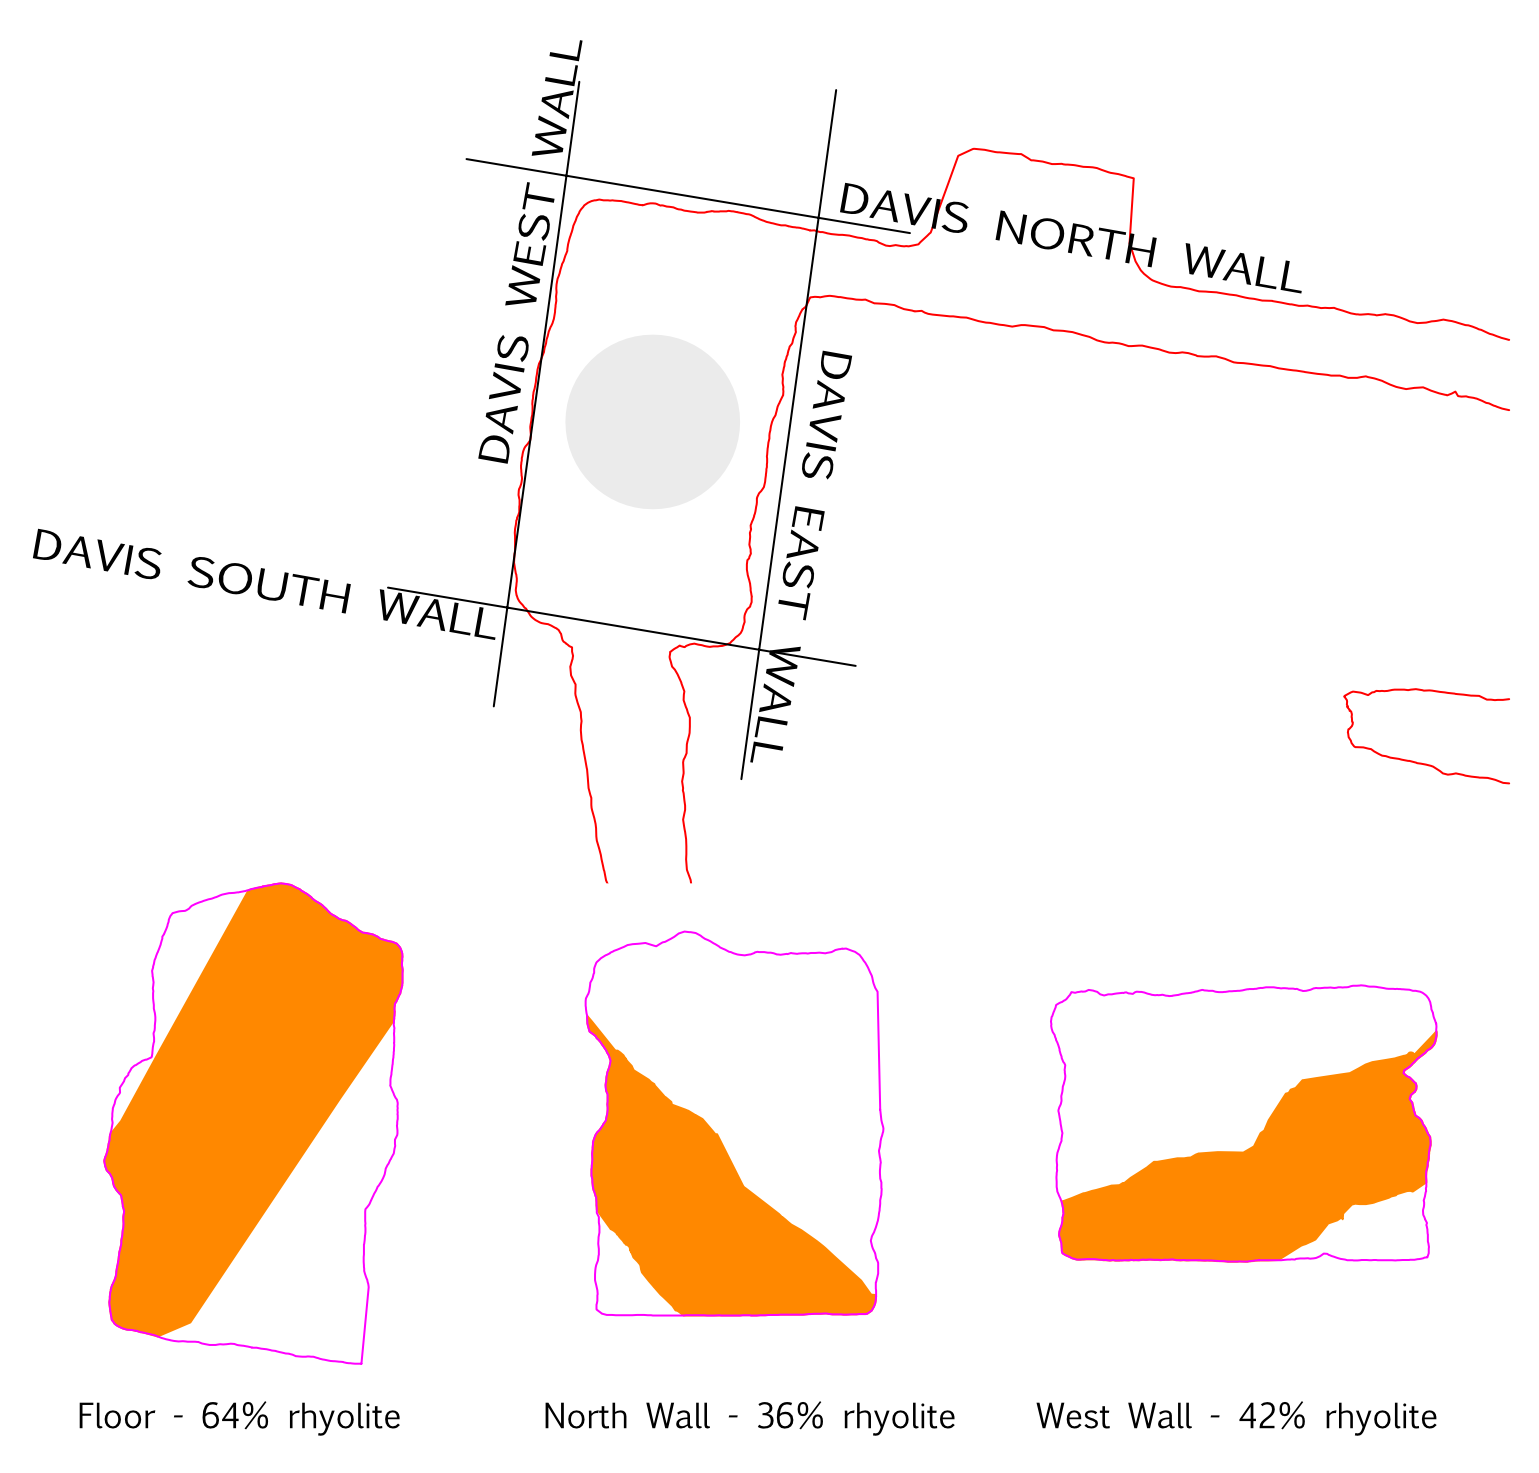
\includegraphics[scale=0.80]{Chapter_3/Figures/Davis_cavern_rhyolite.png}
    \caption[Schematic of the Davis cavern, showing the rhyolite intrusion layers and the position of the water tank with naming conventions.]
    {Diagram of the Davis cavern highlighting the naming conventions of the wall locations and the rhyolite intrusion layers in orange with the estimated percentage coverage of rhyolite. The water tank is marked with a grey circle. The ceiling is estimated at 0\% rhyolite, the south wall at 5\% and the east at 2\% \cite{Heise_2015}. Diagram adapted from \cite{Akerib_2020_gray_measurements}.}
    \label{fig:davis_cavern_walls}
\end{figure}
%

The LZ detectors will be housed within a water tank of height 591 cm and radius 381 cm. Further shielding is provided by 6 octagonal steel plates of 5 cm thickness, inlaid beneath the floor of the water tank with an inverted pyramid hierarchy, directly below the xenon target. The water tank and the steel pyramid are aimed at reducing the environmental radioactivity. Geological and radiometric surveys of the Homestake mine indicate that most rock at the 4,850 level is of the Homestake formation, a metamorphic rock of relatively low uranium and thorium content \cite{Heise_2015}, with additional intrusions of rhyolite segments---an igneous, volcanic, silica-rich rock, with higher natural radioactivity. The estimation of the rhyolite layers as present across the north wall, west wall and the floor are shown in figure \ref{fig:davis_cavern_walls}. The walls and the ceiling of the cavern is lined with a layer of $\sim$12.7 cm thick sprayed concrete (shotcrete) with a thickness variance of factor two. The floor is covered with a 15 cm low-radioactivity concrete with the exception of two rooms at the end of the cavern, away from the water tank. Prior to this measurement, the radiological contents of the rock formation and construction material were measured with high purity germanium (HPGe) screening; these results are shown in table \ref{tab:Davis_cavern_sample_screening}. The table also include two recent measurements of samples collected during this measurement. The following sections will summarise the details of the Davis cavern \gray{} measurements, highlighting the experimental setup, detector calibration, data collection and the results. A more detailed overview of these measurements are presented in \cite{Akerib_2020_gray_measurements}.

\begin{table}[]
\centering
\caption{HPGe screening of rock, shotcrete and gravel samples from the Davis cavern laboratory. The first four materials were radioassayed during construction of the Davis cavern and give the average and range for several samples. The latter two samples were taken during the time of the \gray{} measurements. When not stated, overall uncertainties are estimated to be 10–20\%.}
    \label{tab:Davis_cavern_sample_screening}
    \vspace{1mm}
    \renewcommand{\arraystretch}{1.1}
    \begin{tabular}{lcccc}
    \toprule
    
    \multirow{2}{*}{\textbf{Sample}} & %0
    \textbf{} & %1
    \textbf{$^{40}$K} & %2
    \textbf{$^{238}$U} & %3
    \textbf{$^{232}$Th} \\ %4
    
    \textbf{} & %0
    \textbf{} & %1
    \textbf{[Bq/kg]} & %2
    \textbf{[Bq/kg]} & %3
    \textbf{[Bq/kg]} \\ %4
    
    \hline
    \hline
    
    \multirow{2}{*}{\textbf{Homestake}} & ave. & 297 & 2.7 & 1.3 \\
                                        & range & 31--601 & 0.7--9.5 & 1.0--6.5 \\
    \multirow{2}{*}{\textbf{Rhyolite}}  & ave. & 1291 & 108 & 44 \\
                                        & range & 523--2127 & 99--135 & 7.7--61 \\
    \multirow{2}{*}{\textbf{Concrete}}  & ave. & 381 & 27 & 13 \\
                                        & range & 368--393 & 22–27 & 13–14 \\  
    \multirow{2}{*}{\textbf{Shotcrete}} & ave. & 272 & 23 & 12 \\
                                        & range & 127--393 & 22–28 & 8.1–14 \\ 
    \hline
    \textbf{Shotcrete} & - & 220 \pm 30 & 21 \pm 1 & 11.4 \pm 0.4 \\
    \textbf{Gravel} & - & 35.0 \pm 0.6 & 26.3  \pm 0.1 & 1.7 \pm 0.8 \\
    
    \bottomrule
\end{tabular}
\end{table}


\subsection{Experimental Setup}
\label{secsec:experimental_setup}

The \gray{} flux within the cavern was measured using a thallium-doped sodium iodide (NaI) scintillating crystal ($5 \times 5 \times 5 \; \MathText{inches}$) coupled with a PMT. The detector, manufactured by Harshaw, was connected to a NOMAD 92X-P portable \gray{}-spectroscopy unit. The MAESTRO software was used to produce spectra. A total of 130 lead bricks ($8 \times 4 \times 2 \; \MathText{inches}$) were used in three different configurations for direction specific measurements while shielding away \grays{} from unsought directions, providing at least 8 inches of lead on the sides that were not exposed. A picture of the detector and lead brick configurations in which exposures from above and below are shielding is shown in figure \ref{fig:detector_and_shielding}.
%
\begin{figure}[]
    \centering
    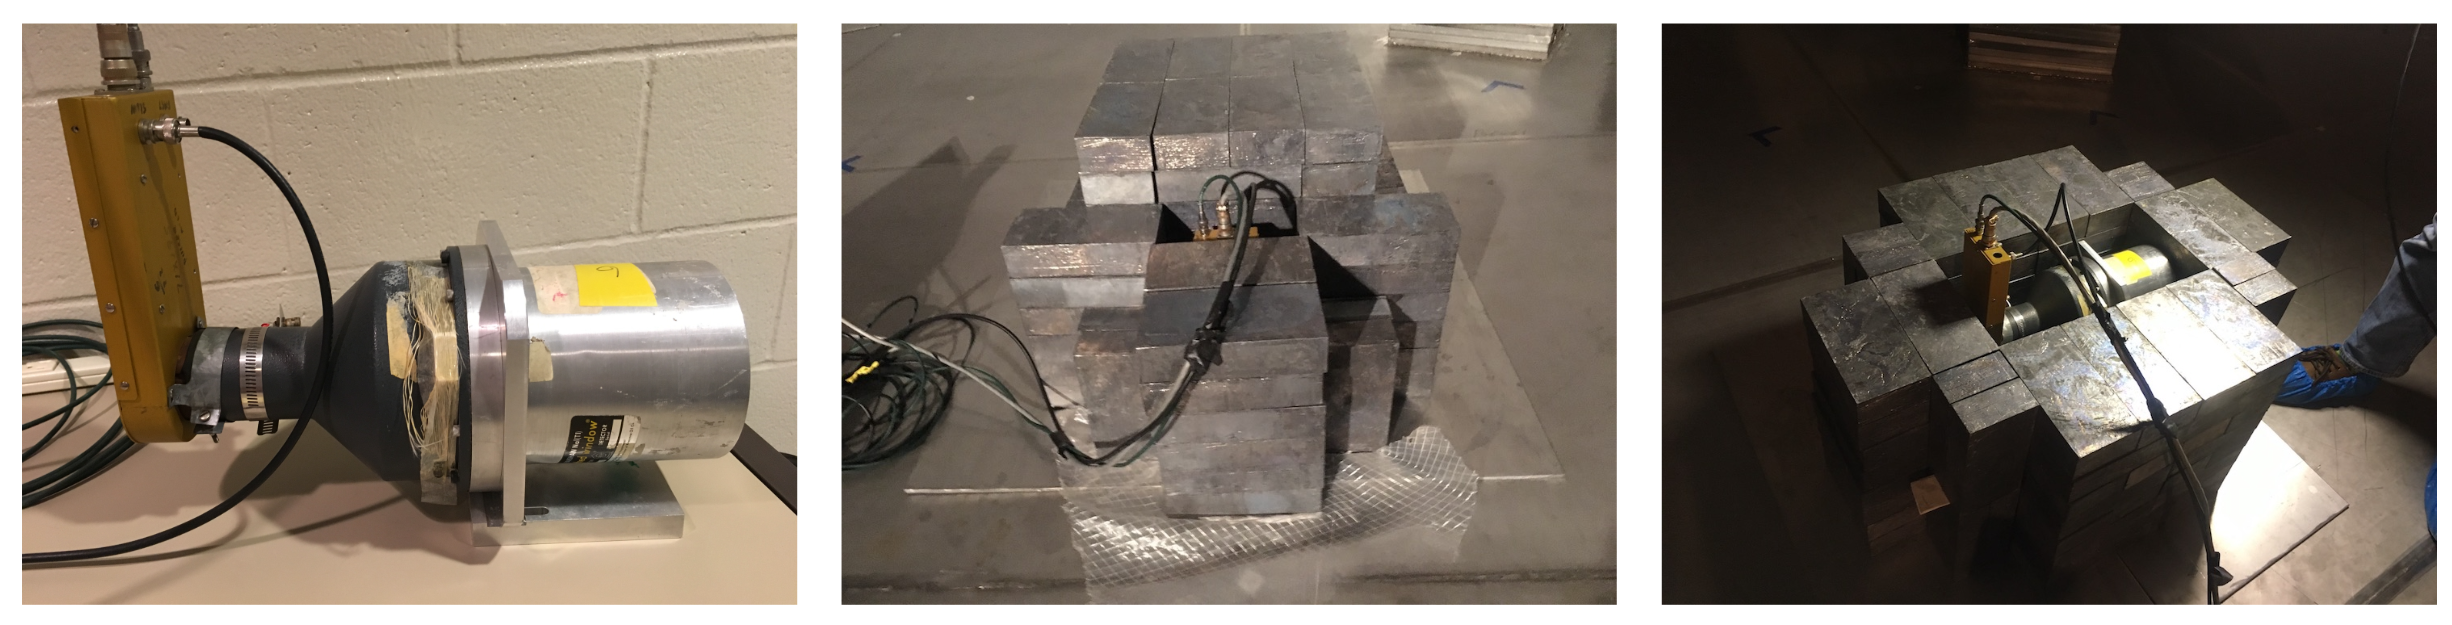
\includegraphics[scale=0.75]{Chapter_3/Figures/Davis_detector_shielding.png}
    \caption[Diagram of the NaI(Tl) crystal detector and the lead shielding used in taking direction specific measurements.]
    {A photograph of the 5-inch NaI(Tl) detector (left), showing the pre-amplifier, PMT and NaI crystal. The right two images are showing the lead shielding configuration in measuring \grays{} from the bottom (centre) and from above (right).}
    \label{fig:detector_and_shielding}
\end{figure}
%

\subsubsection{Detector Calibration and Efficiency}
\label{secsec:calibration_efficiency}


A \CoSZ{} source calibration was performed before each measurement to relate PMT channels to deposited energy and adjust for fluctuations in gain of the NOMAD unit.
Using the 2505 keV peak from \CoSZ{} ensured a dynamic range that fully contained the energy spectrum up to the 2614 keV peak from \TlTZE{}. The detector efficiency and energy resolution were determined by using three calibration sources with their associated energy peaks: \CoSZ{} (1173 keV, 1332 keV, 2505 keV), \CsOTS{} (662 keV) and \TlTZE{} (2614 keV). Each of the energy peaks was fitted with a Gaussian and exponential backgrounds in order to determine the location and resolution of the respective peaks. Calibrations were performed from the same central location within the water tank without shielding. Background measurements from the same location were subtracted from the calibration source spectra to account for \grays{} from the cavern. 

The absolute efficiency of the detector, $\epsilon_{A}$, is given by,
%
\begin{equation}
    \epsilon_{A} = \frac{N(E)}{ATP_{\gamma}(E)}
    \label{eq:detector_eff}
\end{equation}
%
where $N(E)$ is the number of counts in a photopeak of energy $E$, $A$ is the activity of the source, $T$ is the live time and $P_{\gamma}(E)$ is the probability of a single decay producing a \gray{} of energy $E$. $\epsilon_{A}$ is a product of the geometric acceptance due to the fractional solid angle expose of the detector, the \gray{} conversion efficiency within the crystal, and the PMT light collection efficiency. Simulations of calibration sources at varying distances from the detector were performed and source activities were used to calculate the rates in each simulated photopeak. Comparison to data revealed an over-estimation of rates in data, likely as a result of the unaccounted light collection effects in simulations. A correction factor of $0.90 \pm 0.06$ was calculated and applied to further simulations. The resolution, $R$, of each peak was calculated from the full width at half maximum (FWHM) and the energy, $E$, of that peak, using,
%
\begin{equation}
    R = \frac{FWHM}{E} \equiv \frac{\Delta{}E}{E}.
    \label{eq:detector_eff}
\end{equation}
%
The energy dependent resolution scale was then determined by fitting a resolution model, which took into account the light transmission from the scintillating crystal to the photocathode, $\alpha$, statistical fluctuations in photon production, attenuation, conversion and amplification, $\beta$, and the noise contribution, $\gamma$, \cite{An:2016ses}, where,
%
\begin{equation}
    R = \frac{\Delta{}E}{E} \cong \sqrt{\alpha{}^2 + \frac{\beta{}^2}{E} + \frac{\gamma{}^2}{E^{2}}}.
    \label{eq:resolution_model}
\end{equation}
%
The resolution model as applied to the calibrations performed during this measurement are presented in figure \ref{fig:detector_resolution_fit} and were later used to correct the true Monte Carlo energy depositions from the simulations in an effort to directly compare with the data from NaI(Tl) detector.
%
\begin{figure}[]
    \centering
    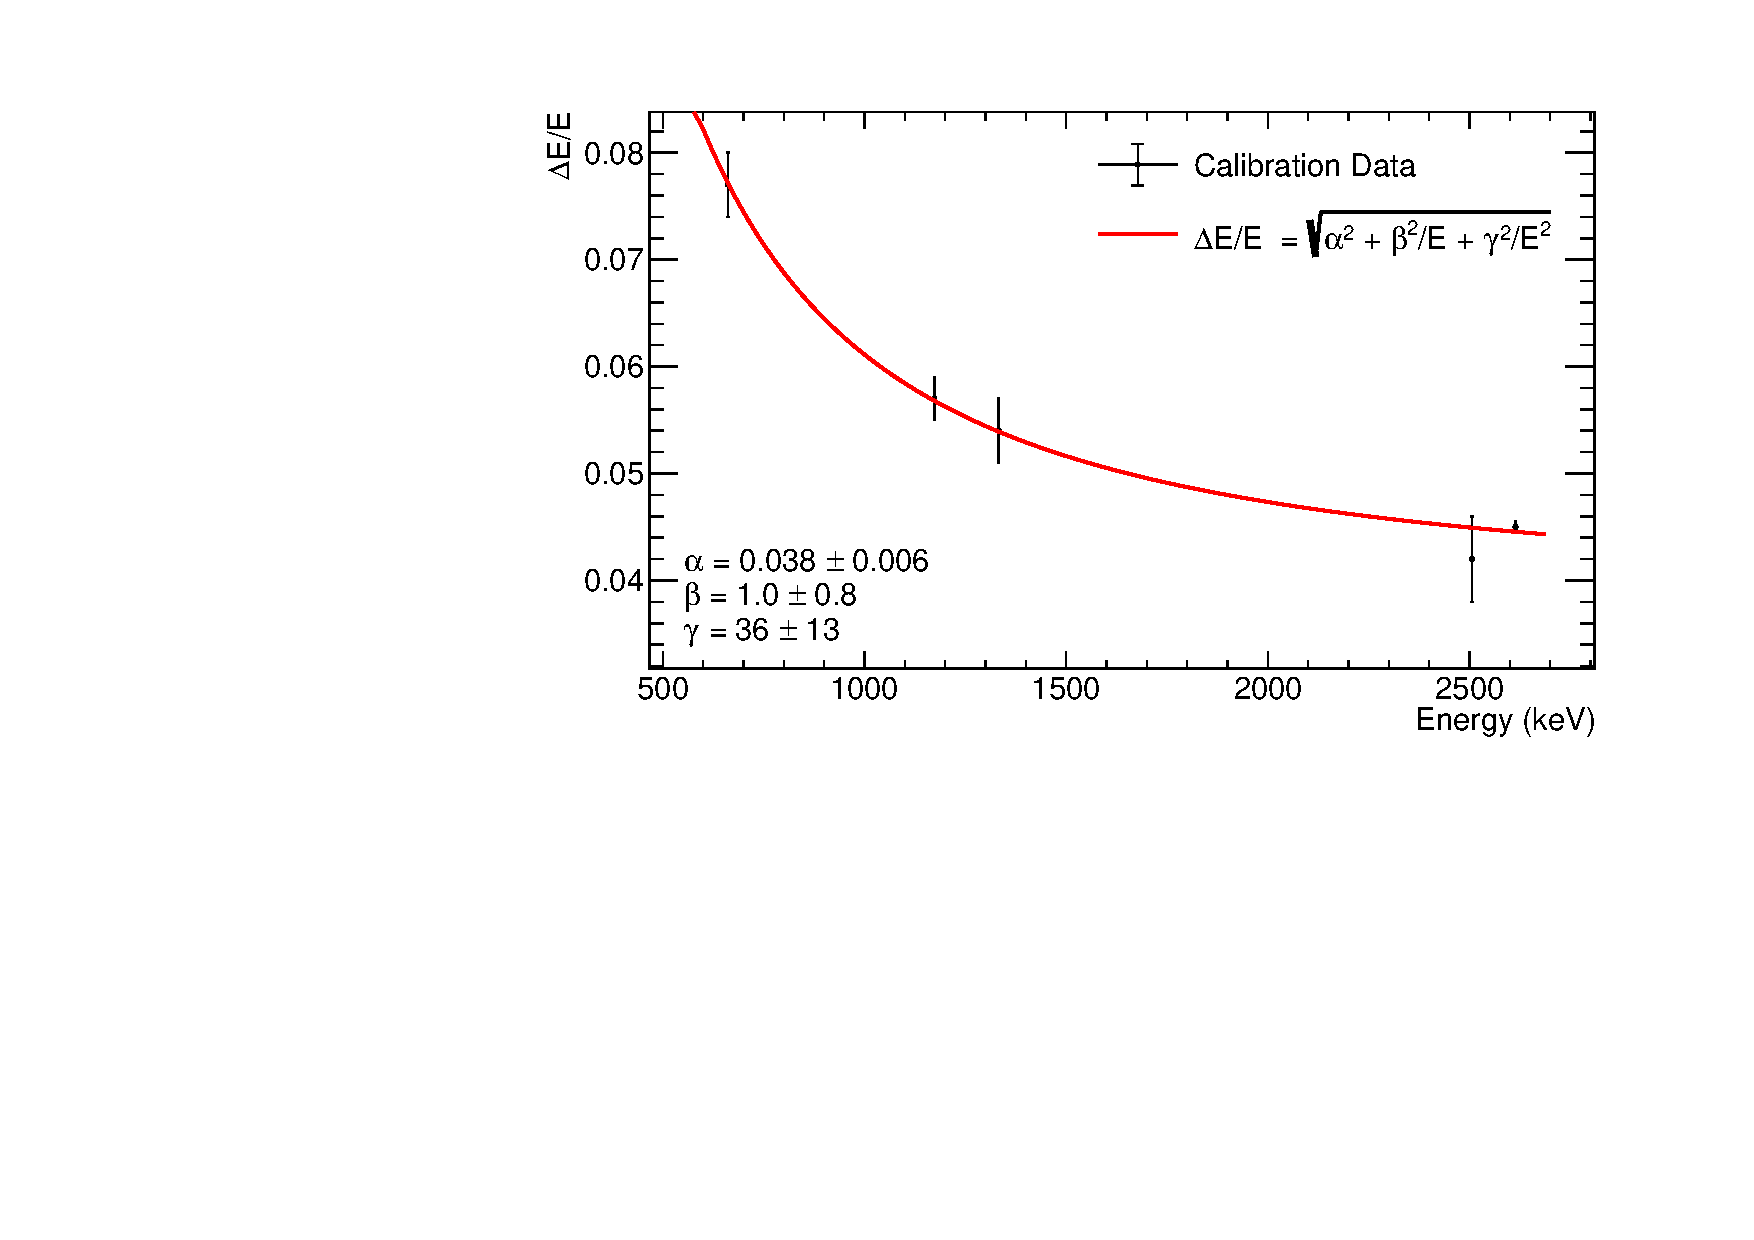
\includegraphics[scale=0.75]{Chapter_3/Figures/NaI_resolution.pdf}
    \caption[Resolution of the NaI(Tl) detector obtained from the calibration source peaks of \CoSZ{}, \CsOTS{} and \ThTTE{}.]
    {Resolution of the NaI(Tl) detector obtained from the calibration source peaks of \CoSZ{}, \CsOTS{} and \ThTTE{}. The fit to data using the resolution model given in equation \ref{eq:resolution_model} is also shown.}
    \label{fig:detector_resolution_fit}
\end{figure}
%


\subsubsection{Data Collection}
\label{secsec:data_collection}

A total of nine measurements were conducted to fully map the \gray{} flux within the Davis cavern, focusing primarily on the flux as seen by the water tank as shown in figure \ref{fig:davis_cavern_layout}. Seven of these were conducted within the water tank; five of which were measurements from the centre of the tank. Locations from the centre consisted of an unshielded measurement (a) and shielded measurements looking down with 30 cm of steel pyramid beneath (f), looking up (g), looking west (h) and looking east (i). The remaining two within the water tank were shielded measurements looking down at the edge (d) and looking down halfway from the centre to the edge with 15 cm of steel pyramid beneath (e). The two measurements outside of the water tank were conducted unshielded in the Upper Davis above the water tank (b) and on the floor of the counting room (c). Measurements looking down within the water tank were aimed at measuring the effectiveness of the steel pyramid, whereas those facing the walls aimed at assessing the asymmetry due to the presence of rhyolite.
%
\begin{figure}[]
    \centering
    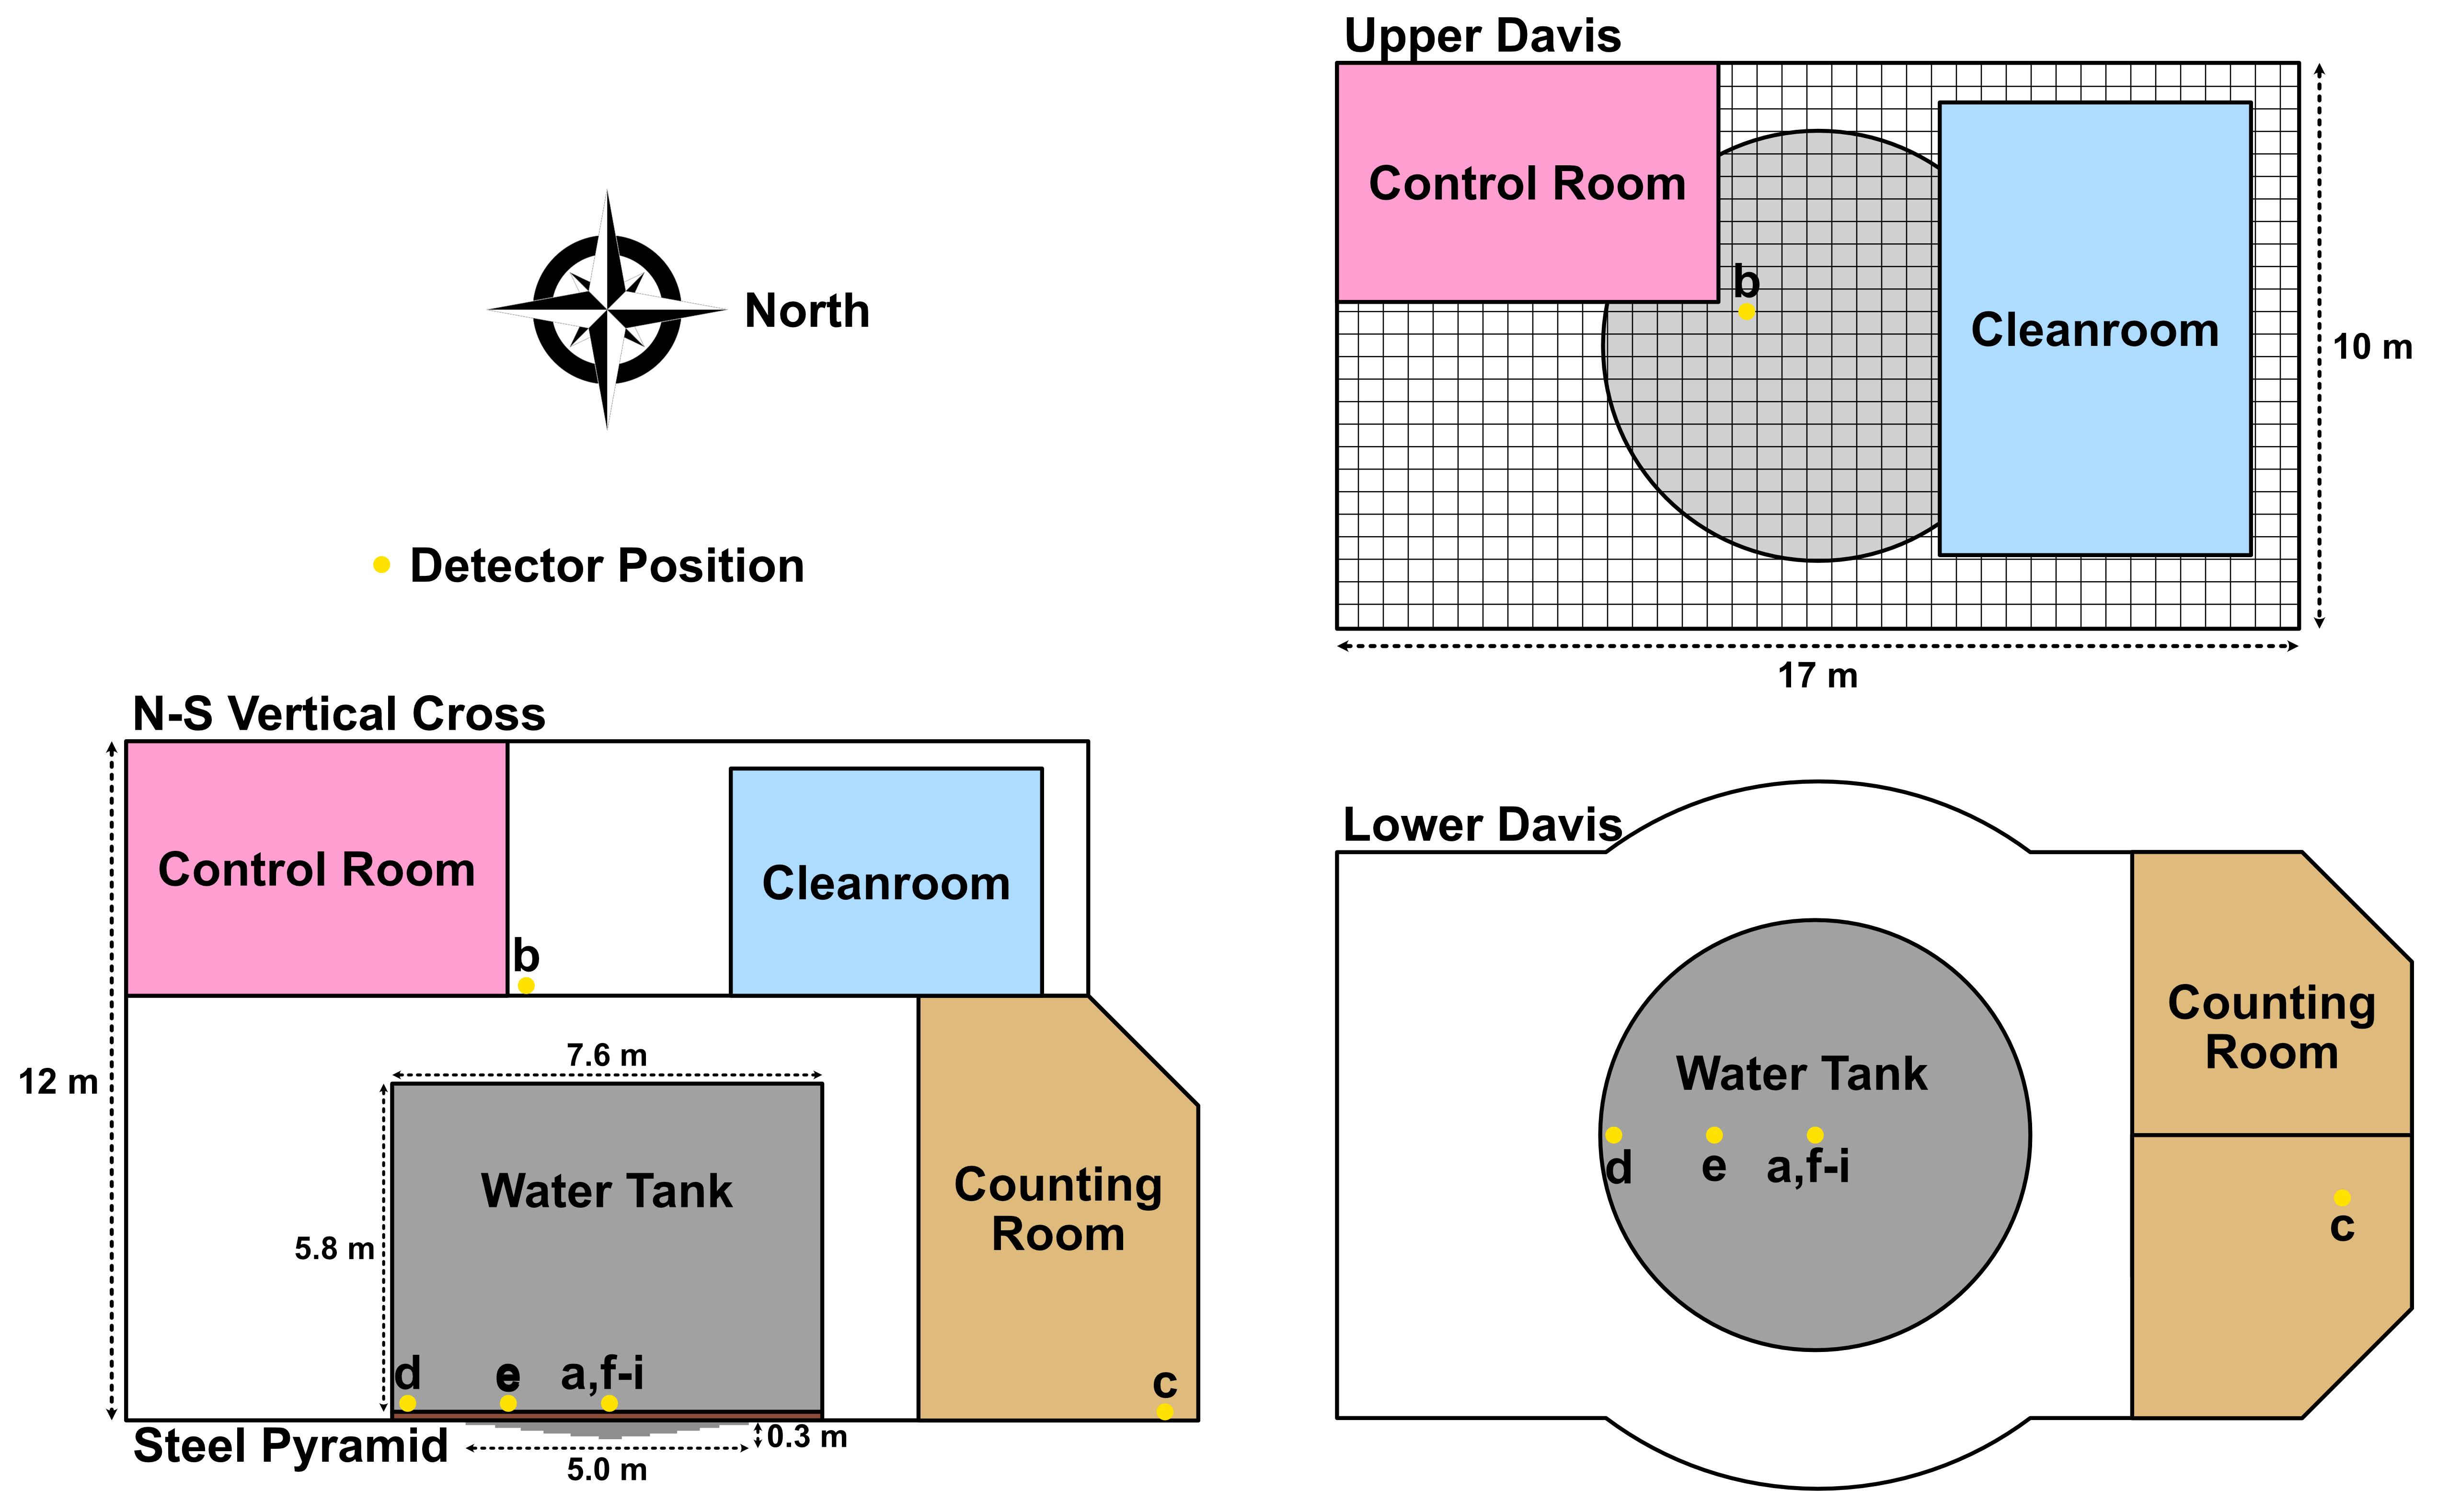
\includegraphics[scale=0.085]{Chapter_3/Figures/Davis_cavern_diagram.jpg}
    \caption[Schematic layout of Davis cavern at the time of the measurement, highlighting key dimensions and the measurement positions with yellow dots.]
    {Schematic layout of Davis cavern at the time of the measurement, highlighting key dimensions and the measurement positions with yellow dots. The labels of the positions directly map to measurement results within table \ref{tab:Davis_cavern_measurement_details}.}
    \label{fig:davis_cavern_layout}
\end{figure}
%
%
\begin{figure}[t!]
    \centering
    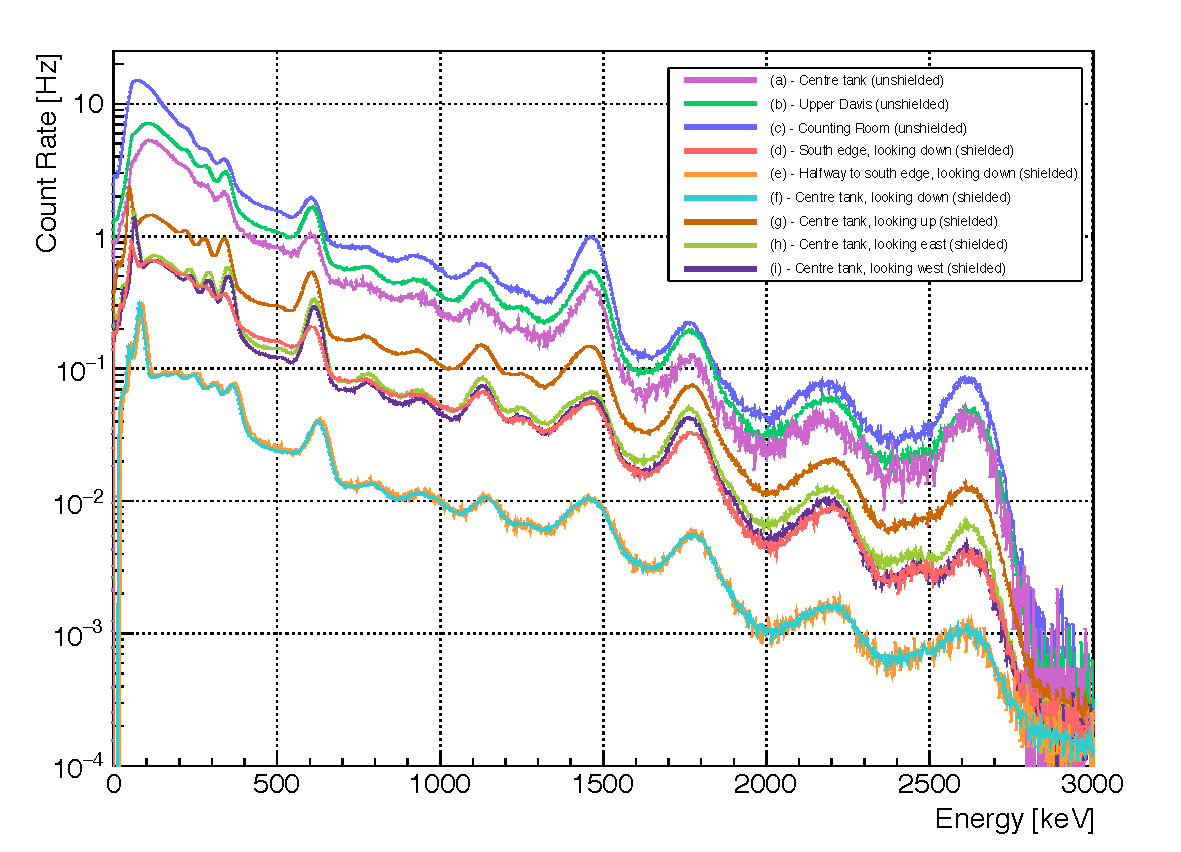
\includegraphics[scale=0.80]{Chapter_3/Figures/Davis_cavern_spectra.pdf}
    \caption[The energy spectra for all nine measurements labeled with their corresponding positions in the energy range 0–3000 keV.]
    {The energy spectra for all nine measurements labeled with their corresponding positions in the energy range 0–3000 keV.}
    \label{fig:davis_cavern_spectra}
\end{figure}
%
The measured energy spectra from all of the 9 positions are shown in figure \ref{fig:davis_cavern_spectra} and their integrated rates, along with differing exposure times and measured ambient radon levels are summaries in table \ref{tab:Davis_cavern_measurement_details}. The lowest rates observed are from two measurements inside of the water tank, at the centre (f) and halfway to the edge (e), both facing down. Despite the much longer exposure time for (f) and the differences in the thickness of pyramid shielding below, the rates observed for these two measurements are comparable. This suggests that the rates observed in these positions are intrinsic to the experimental setup---essentially a background of the experiment, as NaI(Tl) crystals and PMTs are known to have intrinsic \KFZ{}, \UTTE{} and \ThTTT{} contamination \cite{Kim:2014toa}. Measurements facing east and west are comparable in rate, signalling no significant asymmetry due to the difference in rhyolite intrusion within the walls. This may imply that the difference observed in the directional flux ($\sim$ 10\%) may be due to unevenness in shotcrete thickness since the shotcrete is approximately 10 times more radioactive than the Homestake formation in \UTTE{} and \ThTTT{}. The measurement at the edge of the water tank looking down (d) does show a higher rate than both (e, f) suggesting that the steel pyramid is in fact reducing the flux from below. The rates were highest in the east counting room, followed by the upper level of the Davis cavern and the centre of the water tank---all unshielded.

Decays from the \RnTTT{} sub-chain make up a majority of the \grays{} in the \UTTE{} chain, hence the activity of radon within the cavern air must be considered. The average radon concentration, taking into account seasonal dependence in the Davis Campus, is expected to be within 150--310 Bq/m$^3$ \cite{Heise_2015}. However, unusually high radon levels were recorded (measured with an AlphaGuard detector) some of the days, possibly as a result of the air flow and air circulation fluctuations within the mine drift. The recorded levels from an area outside the main entrance to the cavern known as the common corridor during each dataset are also shown in table \ref{tab:Davis_cavern_measurement_details}. Although there may be uncertainties due to the differences in location, the concentrations were significant enough that \grays{} from airborne-radon was included in the analysis.

\begin{table}[h]
\centering
\caption{Dates, live times, radon concentrations and integrated. count rates for each measurement position. The centre of tank measurements were shielded from all directions except the intended direction as stated. Stated uncertainties are Poisson counting errors. Data adapted from \cite{Akerib_2020_gray_measurements}.}
    \label{tab:Davis_cavern_measurement_details}
    \vspace{1mm}
    \renewcommand{\arraystretch}{1.1}
    \begin{adjustbox}{width=\textwidth}
    \begin{tabular}{lcccccc}
    \toprule
    
    \multirow{2}{*}{\textbf{Measurement Position}} & %0
    \multirow{2}{*}{\textbf{Label}} & %1
    \multirow{2}{*}{\textbf{Date}} & %2
    \textbf{Live time} & %3
    \textbf{Ave. \RnTTT{} Act.} & %4
    \textbf{Rate (total)} & %5
    \textbf{Rate (>200 keV)} \\ %6  
    
    \textbf{} & %0
    \textbf{} & %1
    \textbf{} & %2
    \textbf{[hours]} & %3
    \textbf{[Bq/m$^{3}$]} & %4
    \textbf{[Hz]} & %5
    \textbf{[Hz]} \\ %6
    
    \hline
    \hline
    
    Centre of tank (unshielded) & a & 24/10/17 & 4.0 & 422 \pm 34 & 595.7 \pm 0.2 & 386.0 \pm 0.2 \\
    Upper Davis (unshielded) & b & 26/10/17 & 3.6 & 868 \pm 222 & 794.4 \pm 0.2 & 512.0 \pm 0.2 \\
    Counting Room (unshielded) & c & 26/10/17 & 2.1 & 929 \pm 70 & 1355.0 \pm 0.4 & 750.9 \pm 0.3 \\
    South Edge, looking down & d & 16/10/17 & 18.2 & 358 \pm 80 & 94.17 \pm 0.04 & 64.40 \pm 0.03 \\
    Halfway to South Edge, looking down & e & 17/10/17 & 17.9 & 336\pm55 & 17.15 \pm 0.02 & 10.70 \pm 0.01 \\
    Centre of tank, looking down & f & 19/10/17 & 117.0 & 500 \pm 155 & 16.715 \pm 0.006 & 10.427 \pm 0.005 \\
    Centre of tank, looking up & g & 18/10/17 & 20.2 & 372 \pm 76 & 203.57 \pm 0.05 & 139.0 \pm 0.04 \\
    Centre of tank, looking west & h & 24/10/17 & 17.3 & 359 \pm 37 & 95.11 \pm 0.04 & 51.77 \pm 0.03 \\
    Centre of tank, looking east & i & 25/10/177 & 22.3 & 316 \pm 46 & 106.33 \pm 0.4 & 59.14 \pm 0.03 \\
    
    \bottomrule
    \end{tabular}
    \end{adjustbox}
\end{table}


\subsection{Simulation \& Analysis}
\label{secsec:simulations_analysis}

Simulations of the \gray{} background within Davis cavern are performed using the \textsc{BACCARAT} framework, a \textsc{GEANT4} (v.10.03) \cite{Geant4} package developed primarily for LZ background simulations---detailed further in section \ref{sec:LZ_simulation_framework}. Electromagnetic processes were modelled using the \textit{G4EMLivermorePhysics} class, a sub-package that models interactions of \gray{} and electron cross-sections \cite{osti_295438, osti_5691165}, focusing on low energy processes, such as Rayleigh, Compton scattering, bremsstrahlung and the photoelectric effect. 

A custom geometry featuring the cavern, steel pyramids, water tank and the NaI detector was created, with additional shielding geometry, taking into account the three different configurations. The cavern was modelled as a cuboid to have internal dimensions of $20 \times 14 \times 12$ m; slightly larger than stated in figure \ref{fig:davis_cavern_layout} to account for the unevenness of the cavern walls. The cavern walls were defined as a mixture of oxides, primarily SiO$_{2}$, Al$_{2}$O$_{3}$, FeO and water \cite{Mei_2010}. Decays from the \UTTE{} and \ThTTT{} chains and the \KFZ{} decay were all initiated within a 30 cm thick layer of material surrounding the cavern. The \UTTE{} and \ThTTT{} chains were simulated using an event generator developed for LZ background simulations. The generator assumes secular equilibrium and initiates a chain of decays beginning at \UTTE{} or \ThTTT{} and ending at the stable \PbTZS{} or \PbTZE{}, initiating all of the \alpha, \beta and \gamma-decays for the entire chain with correct  energies and branching ratios. Moreover, the \RnTTT{} chain was also simulated within the cavern air and the water tank to account for the elevated levels of radon at the time of the measurement and the rates normalised using the measured concentrations. The simulated dataset recorded energy depositions of the \grays{} within the NaI crystal and further smeared the data using a Gaussian function; accounting for the energy resolution by using the resolution model fit to calibration data as shown in figure \ref{fig:detector_resolution_fit}.

An equivalent of 1 Bq/kg was simulated to calculate the activity necessary for each isotope of interest within the cavern walls to reproduce the rates observed in data. The simplest technique to scale the simulations to data was by fitting a Gaussian to each of the prominent peaks at 1461 keV (\KFZ{}, BR: 10.66\%), 1764 keV (\BiTOF{}, BR: 15.30\%) and 2614 keV (\TlTZE{}, BR: 99.75\%). Focusing on the photopeaks was done in order to select those \grays{} produced near to the surface of the cavern to reduce the effects of the Compton background leaking into each peak. The analysis further focused on \grays{} with energies of 1400 keV or above where the Compton background is less dominant. 
%
\begin{figure}[t!]
    \centering
    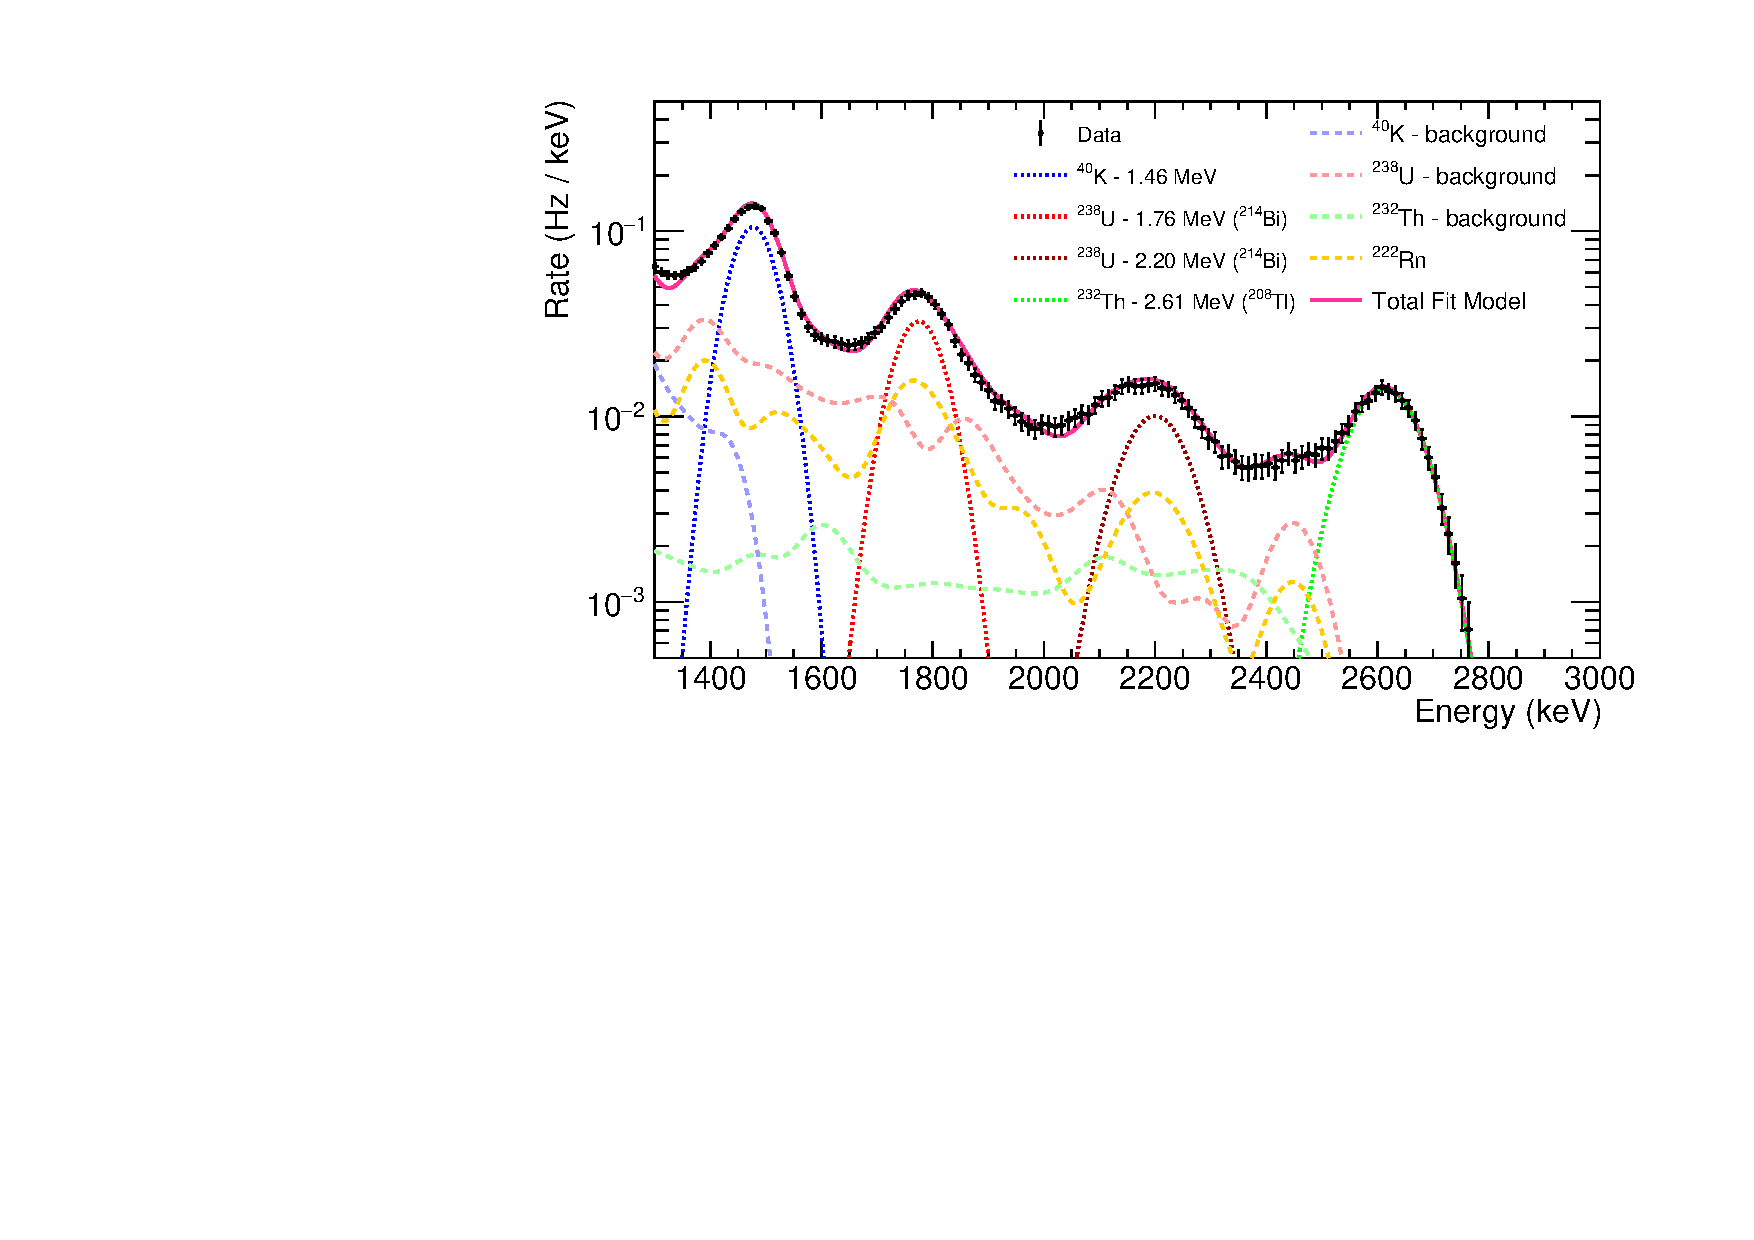
\includegraphics[scale=0.80]{Chapter_3/Figures/Cavern_peak_fits.pdf}
    \caption[Fitted energy spectra for position (a) showing the 1461 keV \KFZ{} peak, 1764 keV and 2204 keV peaks from \UTTE{} and the 2614 keV peak from \ThTTT{}, with background contributions.]
    {Fitted energy spectra for position (a) showing the 1461 keV \KFZ{} peak, 1764 keV and 2204 keV peaks from \UTTE{} and the 2614 keV peak from \ThTTT{}, with background contribution PDFs from less dominant lines, air-borne radon and Compton scattering. Diagram adapted from \cite{Akerib_2020_gray_measurements}.}
    \label{fig:davis_cavern_spectra_fit}
\end{figure}
%
The Compton backgrounds overlaying the peaks of interest contain \grays{} from all energies and peaks from the uranium and thorium chains. To model for this, a background probability distribution function (PDF) was created using the simulated spectra of each isotope with the prominent lines removed and signal PDFs were produced from Gaussian functions with widths constrained within error bars obtained from the resolution function. A background PDF was also constructed for the \RnTTT{} decay chain \grays{} to account for the ambient radon. The fit was constrained by fixing the branching ratio of \BiTOF{}, allowing the rate from radon to  float within 20\% uncertainty due to location dependent uncertainties, and the peak-to-continuum ratio was constrained to float within 20\% of the simulated value for each contribution. An example of the fit to the unshielded data taken in the centre of the water tank is shown in figure \ref{fig:davis_cavern_spectra_fit}.

The corresponding activity of \UTTE{}, \ThTTT{} and \KFZ{} within the wall shell was calculated for each measurement position by using the three isotopic decays by comparison to the simulated rates. The activity for each isotope (denoted by the subscript \textit{i}) and measurement position (denoted by the subscript \textit{p}) is given by
%
\begin{equation}
    A_{i,p} = \frac{R_{i,p} - R^{bkg}}{\epsilon{}R^{sim}_{i,p}},
    \label{eq:resolution_model}
\end{equation}
%
where $R_{i,p}$ is the signal peak in data as determined by the Gaussian fit, $R^{bkg}$ is the internal background rate of the setup as measured in locations e and f, \epsilon{} is the aforementioned efficiency correction determined from calibration and $R^{sim}_{i,p}$ is the simulation normalisation factor calculated using,
%
\begin{equation}
    R^{sim}_{i,p} = \frac{N_{i,p}}{N^{tot}_{i,p}B_{p}M}.
    \label{eq:resolution_model}
\end{equation}
%
Here $N_{i,p}$ is the raw number of counts in a given peak for isotope \textit{i} and position \textit{p}, $N^{tot}_{i,p}$ is the total number of events simulated, $B_{p}$ is the event biasing multiplicative factor and $M$ is the mass of the simulated shell. The event biasing multiplicative factor is as a result of a biasing technique used to increase \gray{} statistics hitting the detector by saving \grays{} on a predefined surface and then propagating a larger quantity onward with the same momentum in a second simulation. The fit results for each peak in activity $A_{i,p}$ are given in table \ref{tab:Davis_cavern_results}.


\subsection{Results \& Discussion}
\label{secsec:results_discussion}

In assuming that each measurement is an independent observation of the same flux within the cavern, the averaged activities across the positions of interest result in $220 \pm 60 \; \MathText{Bq/kg}$ of \KFZ{}, $29 \pm 15 \; \MathText{Bq/kg}$ of \UTTE{} and $13 \pm 3 \; \MathText{Bq/kg}$ of \ThTTT{}. The results from the HPGe screening of the shotcrete samples taken during the measurement indicate activities of $220 \pm 30 \; \MathText{Bq/kg}$ of \KFZ{}, $21 \pm 1 \; \MathText{Bq/kg}$ of \UTTE{} and $11.4 \pm 0.4 \; \MathText{Bq/kg}$ of \ThTTT{}, all of which are in good agreement within uncertainties with the results of this analysis. 

\begin{table}[h]
\centering
\caption
[Results from the fits on the three signature peaks from the \KFZ{}, \UTTE{} and \ThTTT{} decay chains.]
{Results from the fits on the three signature peaks from the \KFZ{}, \UTTE{} and \ThTTT{} decay chains. The best fit activities, $A_{m}$, of the resultant activity within the wall shell from each measurement are given for the positions of interest. The uncertainties are from fit results only, but systematic uncertainties are expected from the simplified simulation geometry. The average values are show at the bottom with their standard deviations. Data adapted from \cite{Akerib_2020_gray_measurements}.}
    \label{tab:Davis_cavern_results}
    \vspace{1mm}
    \renewcommand{\arraystretch}{1.1}
    \begin{adjustbox}{width=\textwidth}
    \begin{tabular}{lc|ccc}
    \toprule
    
    \multirow{2}{*}{\textbf{Measurement Position}} & %0
    \textbf{Label} & %1
    \textbf{$^{40}$K (1461 keV)} & %2
    \textbf{$^{238}$U (1764 keV)} & %3
    \textbf{$^{232}$Th (2614 keV)} \\ %4
    
    \textbf{} & %0
    \textbf{} & %1
    \textbf{ \textit{A$_{p}$} [Bq/kg]} & %2
    \textbf{ \textit{A$_{p}$} [Bq/kg]} & %3
    \textbf{ \textit{A$_{p}$} [Bq/kg]} \\ %4
    
    \hline
    \hline
    
    Centre of tank (unshielded) & a & 285 \pm 1 & 36.9 \pm 0.4 & 15.2 \pm 0.14 \\
    Upper Davis (unshielded) & b & 135 \pm 4 & 10.4 \pm 0.2 & 8.8 \pm 0.1 \\
    Counting Room (unshielded) & c & 264 \pm 1 & 18 \pm 0.2 & 12.2 \pm 0.2 \\
    South Edge, looking down & d & 182 \pm 2 & 31.4\pm0.2 & 16.7 \pm 0.1 \\
    Centre of tank, looking up & g & 214 \pm 1 & 48.4 \pm 0.2 & 9.5 \pm 0.1 \\
    
    \hline
    
    Averaged activities & - & 220 \pm 60 & 29 \pm 15 & 13 \pm 3 \\
    
    \bottomrule
    \end{tabular}
    \end{adjustbox}
\end{table}

However, large variations are observed when taking a closer look at the activities from each measurement; although not fully understood, this could be a result of multiple factors. The first of these could be the uncertainty of the radon concentration within the cavern. The activity of radon used in the simulation were measured outside of the Davis cavern and without a model of the airflow into the cavern, it is difficult to account for this uncertainty. Since most of the \grays{} are emitted from the \RnTTT{} sub-chain, this uncertainty is expected to account for the observed large variations. Furthermore, the simulation does not take into account some of the key features of the cavern, such as the steel grating diving the two floors, walls of the counting room and the control room. Lastly, the variation in different activities may indicate towards a non-uniformity in the concentrations of each isotope spatially within the cavern walls, especially in places where the fluctuations in Shotcrete thickness may lead to \grays{} leaking from the highly active non-uniform Rhyolite layers. Despite the variations between measurements, the results can be used to estimate the background contribution from the Davis cavern for the LZ dark matter experiment.

The overall contribution of \grays{} from the cavern result in a total of $<5$ ER events within the WIMP search region of interest, equating to a small fraction of the total expected ER events, as summarised in table \ref{tab:lz_background_count}. Nevertheless, as discussed in detail in chapter \ref{chap:chap5}, this contribution is taken into account in determining the sensitivity of the LZ experiment to WIMPs. However, it is important to note that Cavern wall \grays{} make up around a third of all backgrounds for the \neutrinolessDoubleBeta{} search in LZ \cite{Akerib_2020_double_beta}.

